
\section{Unity ML-Agents}\label{appendix:mlagents}

% \subsection{Visual Encoders}\label{appendix:visual-encoders}
% todo 

\subsection{PPO Trainer: Hyperparameters}\label{appendix:ppo-trainer}

\begin{longtable}{@{} p{3.5cm} p{2.5cm} p{2.5cm} @{}} \toprule
\textbf{Hyperparemeter}       & \textbf{Default Value} & \textbf{Typical Range} \\ \midrule
visual encoder type         & simple    & - \\ 
normalize                   & false     & - \\
learning rate               & 3e-4      & 1e-5 - 1e-3 \\ 
learning rate schedule      & linear    & linear, constant \\ 
batch size                  &  1024     & 512 - 5120 \\
max steps                   &  500000   & 5e5 - 1e7 \\ 
buffer size                 & 10240     & 2048 - 409600 \\ 
time horizon                &  64       & 32 - 2048  \\
number of layers            &  2        & 1-3 \\
hidden units                &  128      & 32-512 \\
beta                        &  5.0e-3   & 1e-4 - 1e-2  \\
epsilon                     &  0.2      & 0.1 - 0.3  \\
lambda                      &  0.95     & 0.9 - 0.95  \\
number of epochs            & 3         & 3 - 10 \\ \bottomrule
% number of epochs                        & ROSTeat node is running. \\ \cmidrule{1-2} 
% Exceptions             & Image is not RGB \\ \bottomrule
\caption{Default hyperparameters in PPO trainer, taken from \cite{github-unity-mlagents-toolkit}} \label{tab:default-hyperparameters}
% \\
\end{longtable}

\newpage

\subsection{Unity Project Class Diagram}

% TODO insert C\# model diagram.

\begin{figure}[!ht]
    \centering
    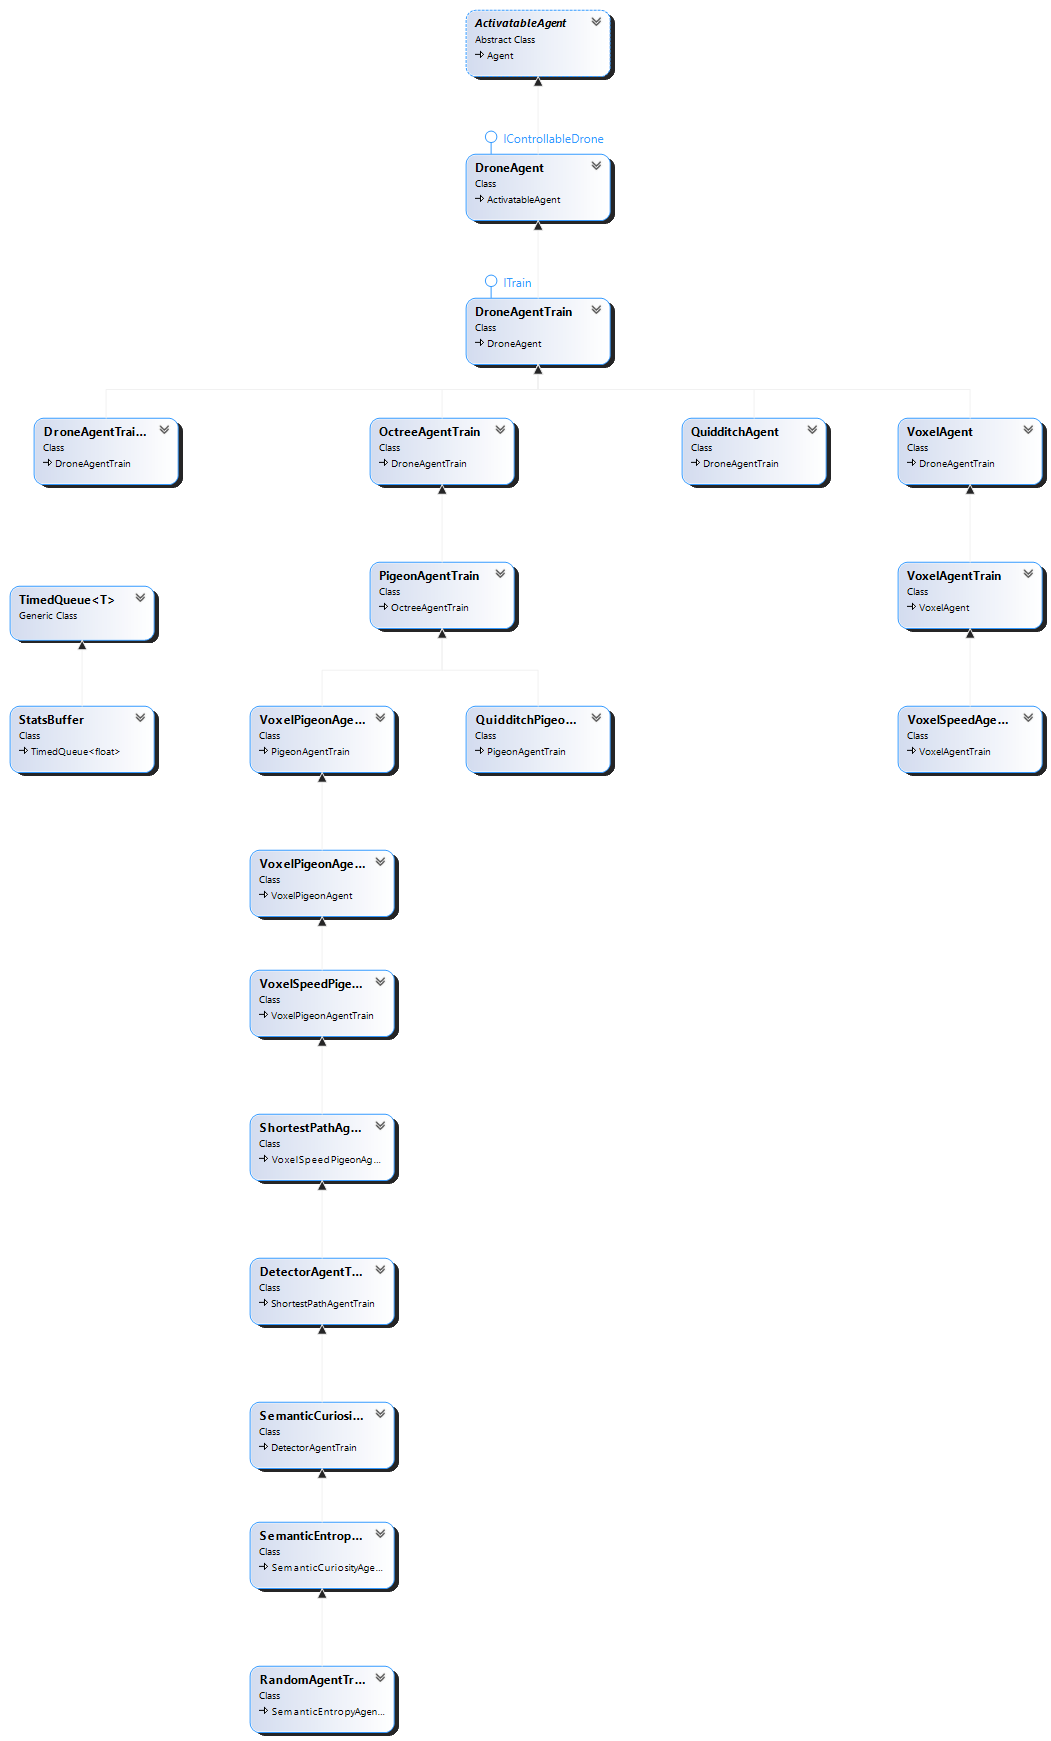
\includegraphics[width=0.8\textwidth]{images/ClassDiagram2.png}
    \caption{Class Diagram for the C\# implementation for this thesis shows the hierarchical behavior inheritance in the implementation of the agents. Generated using Visual Studio 2019.}
    \label{fig:classdiagram}
\end{figure}


\newpage
% \subsection{Example Training Configuration File}\label{appendix:ppo-trainer}
% \newpage
\begin{multicols}{2}
[
\subsection{Example Training Configuration File}\label{appendix:ppo-trainer}
% All human things are subject to decay. And when fate summons, Monarchs must obey.
]
\begin{minted}[
    gobble=4,
    frame=single,
    linenos
  ]{yaml}
    # config file: run63++100.yaml
    behaviors:
      Drone:
        trainer_type: ppo
        hyperparameters:
          batch_size: 1024
          buffer_size: 10240
          learning_rate: 0.0003
          beta: 0.01
          epsilon: 0.2
          lambd: 0.95
          num_epoch: 3
          learning_rate_schedule: linear
        network_settings:
          normalize: false
          hidden_units: 256
          num_layers: 2
          vis_encode_type: simple
          # no lstm
        reward_signals:
          extrinsic:
            gamma: 0.99
            strength: 1.0
          curiosity:
            gamma: 0.99
            strength: 0.02
            network_settings:
              hidden_units: 256
            learning_rate: 0.0003
        keep_checkpoints: 5
        max_steps: 20000000
        time_horizon: 64
        summary_freq: 30000
\end{minted}
\columnbreak

\begin{minted}[
    gobble=4,
    frame=single,
    % linenos
  ]{yaml}
    environment_parameters:
      # 0:base, 1:open, 2:fire, 3:forest
      EnvironmentType: 0 
      steuernModus: 1
      m_EnableVFX: 0
      m_EnableTrainDebuggingLogs: 0
      # base
      m_TrainMovingForward: 1
      m_TrainTargetSpeed: 1
      # octree
      leafNodeSize: 4
      m_AddOctreeObservations: 0
      m_TrainOctreeDiscovery: 0
      m_TrainLingerPolicy: 0
      m_AddPigeonObservations: 0
      # voxel
      m_TrainVoxelCollection: 1
      allowedToSeeVoxels: 1
      m_VoxelRewardStrength: 1
      NormalizeVoxelReward: 0 
      # enabled for all voxel-behaviors
      m_SpeedSensitivityToTargetsInFOV: 1
      # shortest
      m_AddShortestPathObservations: 0
      m_TrainShortestPath: 0
      # detector
      m_LoadDetector: 0
      m_AddDetectorObservations: 0
      m_TrainObjectDetectionMaximization: 0
      NormalizeDetectionsReward: 1
      # curiosity
      m_AddSemanticCuriosityObservations: 0
      m_TrainSemanticCuriosity: 0
      # entropy
      m_AddSemanticEntropyObservations: 0
      m_TrainSemanticEntropy: 0
\end{minted}

\end{multicols}


\newpage

\subsection{Agent Behaviors UI}  \label{appendix:agents_explanations}


% \begin{figure}[!ht]
%     \centering
%     \subfigure{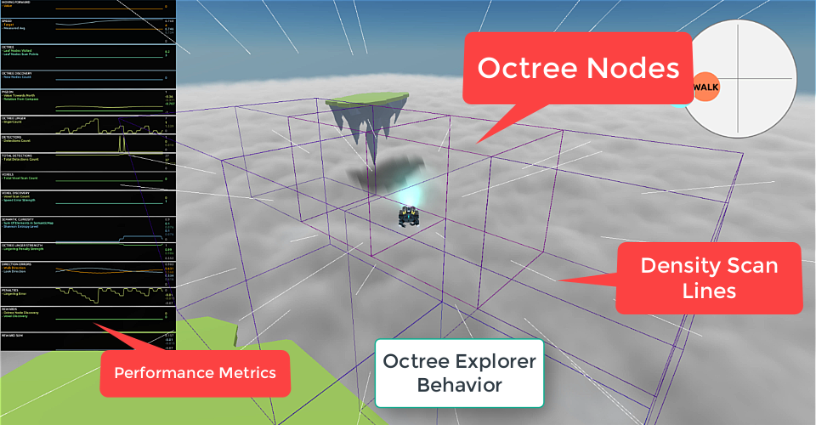
\includegraphics[width=0.49\textwidth]{images/unity-environments-training-behavior-octree2.png}} 
%     \subfigure{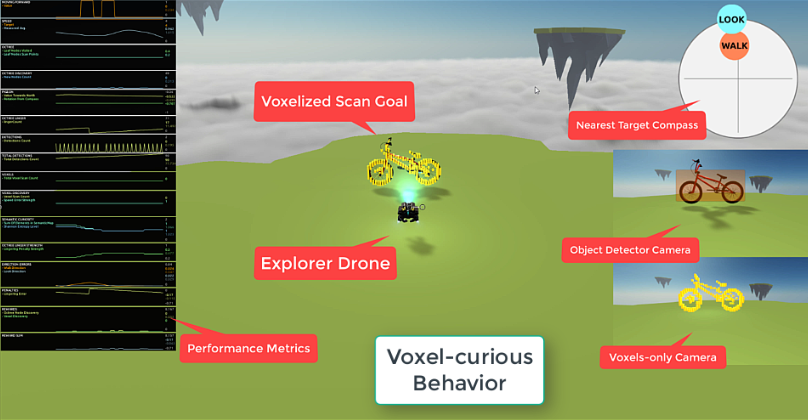
\includegraphics[width=0.49\textwidth]{images/unity-environments-training-behavior-voxel.png}} 
%     \caption{Sample 3D assets for scenario proposals. Taken from \cite{unity-asset-store}.}
%     \label{fig:unity-my-unity-behaviors}
% \end{figure}

\begin{figure}[!ht]
    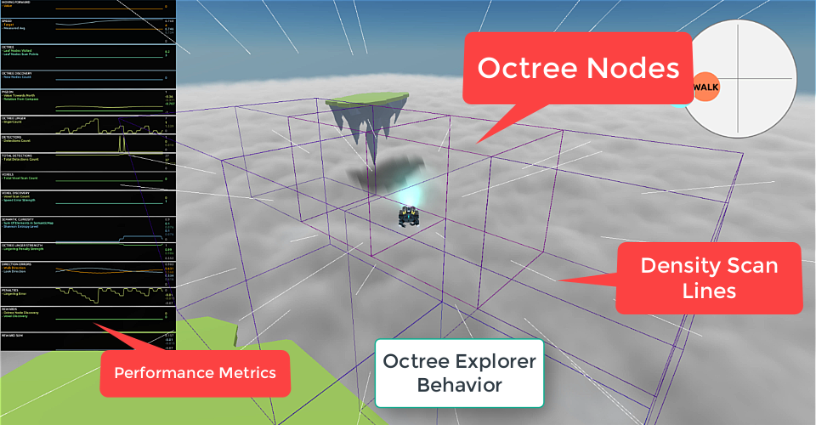
\includegraphics[width=1\textwidth]{images/unity-environments-training-behavior-octree2.png}
    \caption{Octree nodes and agent perspective in the training environment.}
\end{figure}

\begin{figure}[!ht]
    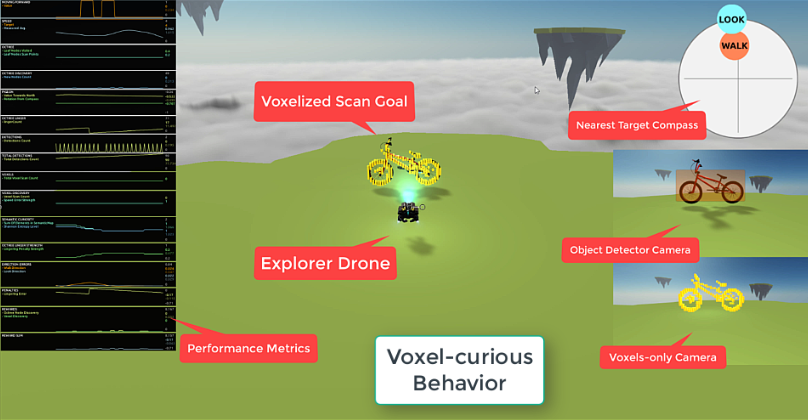
\includegraphics[width=1\textwidth]{images/unity-environments-training-behavior-voxel.png}
    \caption{Agent perspective in the training environment of the voxelized scan goal, including the nearest object compass, object detector camera, voxels-only camera and performance metrics.
    }
    \end{figure}

\newpage 
\subsection{Influence of Variables}  \label{appendix:agent_variables_influence}
    These charts also suggest that the lingering penalty has a smaller influence on the performance of agents, regardless of different strengths of the voxel reward. 

   \begin{figure}[!h]
        \centering
        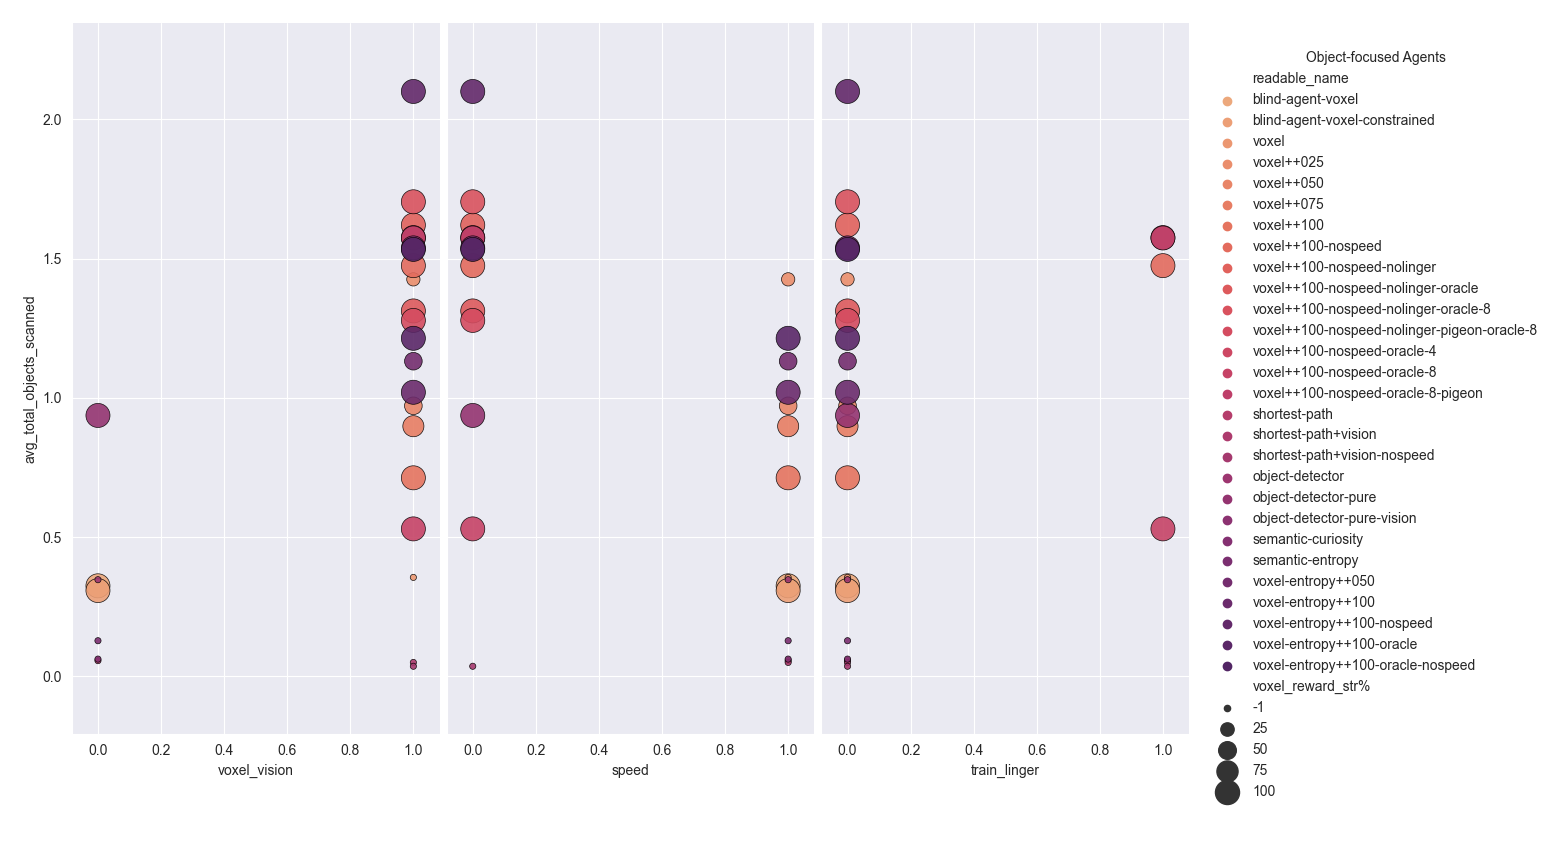
\includegraphics[width=1\textwidth]{images/results_variables_obj3_detailed.png} 
        \caption{Comparison of the influence of relevant variables on the total amount of objects scanned for all object-focused runs. The variables for \textit{pigeon} and \textit{pathak} are always set to 1 (active).}
        \label{fig:results_variables_obj}
        \end{figure}
        


   \begin{figure}[!h]
        \centering
        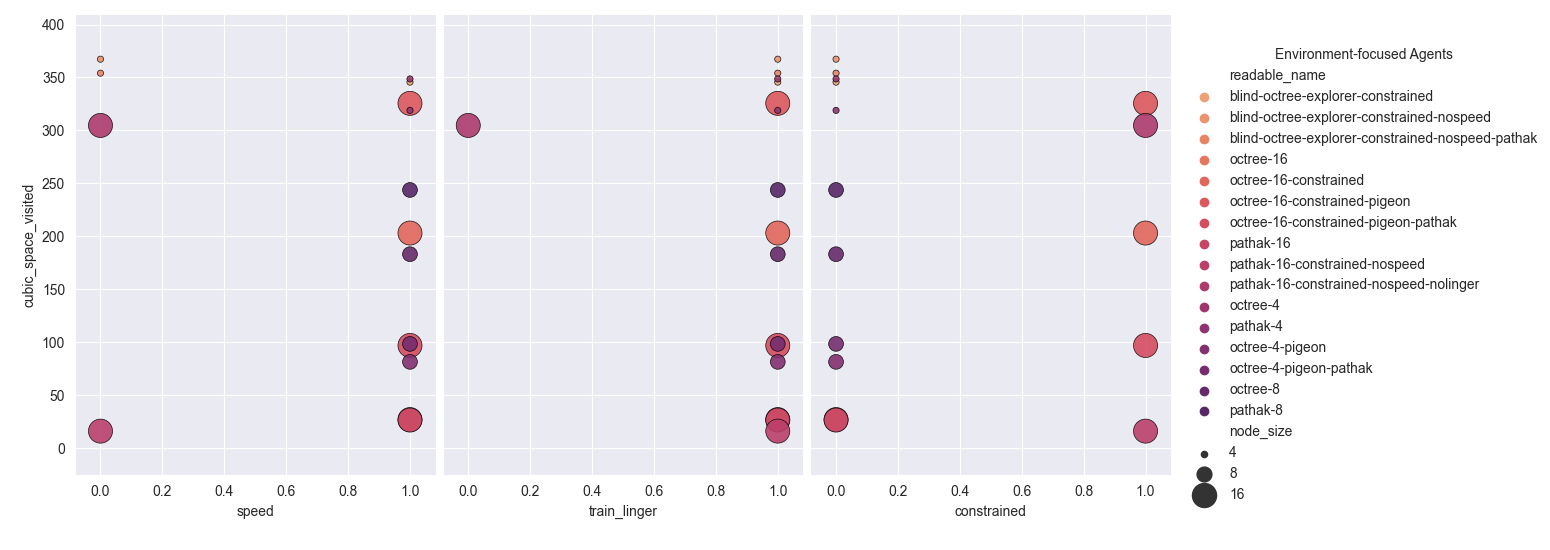
\includegraphics[width=1\textwidth]{images/results_variables_env3.png} 
        \caption{Comparison of the influence of relevant variables on the visited volume for all environment-focused runs.}
        \label{fig:results_variables_obj}
        \end{figure}
        
        

\newpage
\subsection{In-depth Metrics}\label{appendix:indepth-metrics}
The following in-depth metrics were collected per agent

% The full list of in-depth metrics is listed below:
    \begin{multicols}{3}
\begin{itemize}
    \item name
    \item speed
    \item linger
    \item pigeon
    \item pathak
    \item constrained
    \item node\_size
    \item train\_octree\_discovery
    \item train\_voxel\_discovery
    \item voxel\_reward\_str
    \item voxel\_vision
    \item oracle
    \item train\_entropy
    \item sac
    \item n\_leafNodes
    \item n\_leafNodes\_y
    \item leafNodeVolume
    \item \%leafNodesExplored
    \item \%scanNodesExplored
    \item visual\_analysis %\_confirms\_best
    \item \%episode\_length
    \item avg\_total\_objects\_scanned
\end{itemize}
\end{multicols}


\subsection{Naming}

Following what was explained in Section \ref{chap:4:behaviors}, the run names that have a number such as \textit{run63++025} indicate that the voxel reward has a weight factor of 25\%, whereas \textit{run63++100} provides the agent a 100\% of the voxel reward. This allowed the analysis of different influences of voxel reward values and their impact on the agent's behavior. Furthermore, \textit{-constrained} indicates that the training environment manager will not reset the episode if the agent hits a boundary wall.

Similarly, following what was presented in equation \ref{eu_lingeringpenaltystrength}, agents that are labeled with the -entropy suffix, such as \textit{voxel-entropy++100}, observe the variable \textit{lingering-penalty-strength} and accordingly modify the lingering penalty at each timestep. This should enable agents to navigate longer in locations with high entropy. In contrast, agents with the suffix \textit{-noTrainEntropy} only introduce observe the strength factor but do not modify the lingering penalty. 

Given its performance, the baseline for mixed-focus agents is also known as \textit{voxel-entropy-nospeed-octree-pigeon-pathak}. 
As mentioned in \ref{appendix:agents_explanations}, the variants of this baseline are created varying the octree leaf node size, the lingering penalty and the "noTrainEntropy" suffix, which refers to agents that receive entropy observations yet do not modify the lingering penalty based on the entropy levels.

The following tables further explain the names of each agent in terms of rewards and observations.

\begin{sidewaystable}
\subsubsection{Agent Definitions by Observations}
 
    % \hspace{-\marginparsep}    
    % \hspace{-0.5\marginparwidth}
  
    \begin{longtable}{l|cccccccc|l}
    \cline{2-9}
     & \multicolumn{8}{c|}{Obs. per Baseline} &  \\ \hline
    \multicolumn{1}{|l|}{Baseline} & \multicolumn{1}{c|}{\begin{tabular}[c]{@{}c@{}}Octree \\ Obs.\end{tabular}} & \multicolumn{1}{c|}{\begin{tabular}[c]{@{}c@{}}Voxel \\ Vision\end{tabular}} & \multicolumn{1}{c|}{\begin{tabular}[c]{@{}c@{}}Pigeon\\ Obs.\end{tabular}} & \multicolumn{1}{l|}{\begin{tabular}[c]{@{}l@{}}Speed \\ Sensitivity \\ to FOV\end{tabular}} & \multicolumn{1}{c|}{\begin{tabular}[c]{@{}c@{}}Shortest \\ Path\\  Obs.\end{tabular}} & \multicolumn{1}{c|}{\begin{tabular}[c]{@{}c@{}}Detector \\ Obs.\end{tabular}} & \multicolumn{1}{c|}{\begin{tabular}[c]{@{}c@{}}Semantic \\ Curiosity \\ Obs.\end{tabular}} & \begin{tabular}[c]{@{}c@{}}Semantic \\ Entropy \\ Obs.\end{tabular} & \multicolumn{1}{l|}{Comment} \\ \hline
    
    \multicolumn{1}{|l|}{Random Walk} & \multicolumn{1}{c|}{} & \multicolumn{1}{c|}{} & \multicolumn{1}{c|}{} & \multicolumn{1}{c|}{} & \multicolumn{1}{c|}{} & \multicolumn{1}{c|}{} & \multicolumn{1}{c|}{} &  & \multicolumn{1}{l|}
    {Simple agent with obs: speed and position in 3D space.} \\ \hline
    
    \multicolumn{1}{|l|}{Octree Agent} & \multicolumn{1}{c|}{\emoji{x}} & \multicolumn{1}{c|}{} & \multicolumn{1}{c|}{\emoji{x}} & \multicolumn{1}{c|}{} & \multicolumn{1}{c|}{} & \multicolumn{1}{c|}{} & \multicolumn{1}{c|}{} &  & \multicolumn{1}{l|}
    {DA with discovered octree nodes count each timestep.} \\ \hline
    
    \multicolumn{1}{|l|}{Voxel (R\_VOX norm)}  & \multicolumn{1}{c|}{} & \multicolumn{1}{c|}{\emoji{x}} & \multicolumn{1}{c|}{} & \multicolumn{1}{c|}{\emoji{x}} & \multicolumn{1}{c|}{} & \multicolumn{1}{c|}{} & \multicolumn{1}{c|}{} &  & \multicolumn{1}{l|}{
    DA that observes voxels with a normalized reward.} \\ \hline
    
    \multicolumn{1}{|l|}{Voxel (R\_VOX str: 0.25)}  & \multicolumn{1}{c|}{} & \multicolumn{1}{c|}{\emoji{x}} & \multicolumn{1}{c|}{} & \multicolumn{1}{c|}{\emoji{x}} & \multicolumn{1}{c|}{} & \multicolumn{1}{c|}{} & \multicolumn{1}{c|}{} &  & \multicolumn{1}{l|}{
    DA that observes voxels with a reward strength of 25\%} \\ \hline
    
    \multicolumn{1}{|l|}{Voxel (R\_VOX str: 0.50)}   & \multicolumn{1}{c|}{} & \multicolumn{1}{c|}{\emoji{x}} & \multicolumn{1}{c|}{} & \multicolumn{1}{c|}{\emoji{x}} & \multicolumn{1}{c|}{} & \multicolumn{1}{c|}{} & \multicolumn{1}{c|}{} &  & \multicolumn{1}{l|}{
    DA that observes voxels with a reward strength of 50\%} \\ \hline
    
    \multicolumn{1}{|l|}{Voxel (R\_VOX str: 0.75)}  & \multicolumn{1}{c|}{} & \multicolumn{1}{c|}{\emoji{x}} & \multicolumn{1}{c|}{} & \multicolumn{1}{c|}{\emoji{x}} & \multicolumn{1}{c|}{} & \multicolumn{1}{c|}{} & \multicolumn{1}{c|}{} &  & \multicolumn{1}{l|}{
    DA that observes voxels with a reward strength of 75\%} \\ \hline
    
    \multicolumn{1}{|l|}{Voxel (R\_VOX str: 1.00)}   & \multicolumn{1}{c|}{} & \multicolumn{1}{c|}{\emoji{x}} & \multicolumn{1}{c|}{} & \multicolumn{1}{c|}{\emoji{x}} & \multicolumn{1}{c|}{} & \multicolumn{1}{c|}{} & \multicolumn{1}{c|}{} &  & \multicolumn{1}{l|}{
    DA that observes voxels with a reward strength of 100\%} \\ \hline
    
    \multicolumn{1}{|l|}{Shortest Path}  & \multicolumn{1}{c|}{} & \multicolumn{1}{c|}{} & \multicolumn{1}{c|}{} & \multicolumn{1}{c|}{\emoji{x}} & \multicolumn{1}{c|}{\emoji{x}} & \multicolumn{1}{c|}{} & \multicolumn{1}{c|}{} &  & \multicolumn{1}{l|}{
    DA with walk angle and look angle to target.} \\ \hline

    \multicolumn{1}{|l|}{Shortest Path + Vision}  & \multicolumn{1}{c|}{} & \multicolumn{1}{c|}{\emoji{x}} & \multicolumn{1}{c|}{} & \multicolumn{1}{c|}{\emoji{x}} & \multicolumn{1}{c|}{} & \multicolumn{1}{c|}{} & \multicolumn{1}{c|}{} &  & \multicolumn{1}{l|}{
    DA with voxel vision.} \\ \hline
    
    \multicolumn{1}{|l|}{Object Detection} & \multicolumn{1}{c|}{} & \multicolumn{1}{c|}{} & \multicolumn{1}{c|}{} & \multicolumn{1}{c|}{\emoji{x}} & \multicolumn{1}{c|}{} & \multicolumn{1}{c|}{\emoji{x}} & \multicolumn{1}{c|}{} &  & \multicolumn{1}{l|}{
    Simple agent with input from object detector.} \\ \hline

    \multicolumn{1}{|l|}{Object Detection + pure} & \multicolumn{1}{c|}{} & \multicolumn{1}{c|}{} & \multicolumn{1}{c|}{} & \multicolumn{1}{c|}{\emoji{x}} & \multicolumn{1}{c|}{} & \multicolumn{1}{c|}{} & \multicolumn{1}{c|}{} &  & \multicolumn{1}{l|}{
    Simple agent without speed constraint.} \\ \hline
    
    \multicolumn{1}{|l|}{Semantic Curiosity} & \multicolumn{1}{c|}{} & \multicolumn{1}{c|}{} & \multicolumn{1}{c|}{} & \multicolumn{1}{c|}{\emoji{x}} & \multicolumn{1}{c|}{} & \multicolumn{1}{c|}{} & \multicolumn{1}{c|}{\emoji{x}} &  & \multicolumn{1}{l|}{
    DA with rationalized class density each timestep.} \\ \hline
    
    \multicolumn{1}{|l|}{Semantic Entropy}& \multicolumn{1}{c|}{} & \multicolumn{1}{c|}{} & \multicolumn{1}{c|}{} & \multicolumn{1}{c|}{\emoji{x}} & \multicolumn{1}{c|}{} & \multicolumn{1}{c|}{} & \multicolumn{1}{c|}{} &  & \multicolumn{1}{l|}{
    DA with lingering penalty strength present reduction.} \\ \hline
    
    \multicolumn{1}{|l|}{Explorer (R\_VOX str: 0.5)}  & \multicolumn{1}{c|}{\emoji{x}} & \multicolumn{1}{c|}{\emoji{x}} & \multicolumn{1}{c|}{\emoji{x}} & \multicolumn{1}{c|}{\emoji{x}} & \multicolumn{1}{c|}{} & \multicolumn{1}{c|}{} & \multicolumn{1}{c|}{} & \emoji{x} & \multicolumn{1}{l|}
    {DA as above. Voxel reward strength of 50\%} \\ \hline
    
    \multicolumn{1}{|l|}{Explorer (R\_VOX str: 1.0)} & \multicolumn{1}{c|}{\emoji{x}} & \multicolumn{1}{c|}{\emoji{x}} & \multicolumn{1}{c|}{\emoji{x}} & \multicolumn{1}{c|}{\emoji{x}} & \multicolumn{1}{c|}{} & \multicolumn{1}{c|}{} & \multicolumn{1}{c|}{} & \emoji{x} & \multicolumn{1}{l|}
    {DA as above. Voxel reward strength of 100\%} \\ \hline
    
    \caption{Diverse agent behavior variants and the observations they receive. "DA" stands for Derived Agent. All agents observe their own information, such as 3D position, orientation, etc.}
    \label{appendix:baselines_observations}
    
    \end{longtable}%

        % \usepackage{graphicx}
       
\end{sidewaystable}

\begin{sidewaystable}
\subsubsection{Agent Definitions by Rewards}    

 
    % \hspace{-\marginparsep}    
    % \hspace{-0.5\marginparwidth}
  
    \begin{longtable}{l|ccccccc|l}
    \cline{2-8}
             & \multicolumn{7}{c|}{Trained Functions} &  \\ \hline
            %  \multicolumn{1}{c|}{\begin{tabular}[c]{@{}c@{}} Moving \\ Forward\end{tabular}}
            \multicolumn{1}{|l|}{Baseline}  & \multicolumn{1}{c|}{\begin{tabular}[c]{@{}c@{}} Speed\end{tabular}} & \multicolumn{1}{c|}{\begin{tabular}[c]{@{}c@{}}  Octree \\ Nodes\\  Discovery\end{tabular}} & \multicolumn{1}{c|}{\begin{tabular}[c]{@{}c@{}} Voxel \\ Discovery\end{tabular}} & \multicolumn{1}{c|}{\begin{tabular}[c]{@{}c@{}} Shortest \\ Path\end{tabular}} & \multicolumn{1}{c|}{\begin{tabular}[c]{@{}c@{}} Object \\ Detection\end{tabular}} & \multicolumn{1}{c|}{\begin{tabular}[c]{@{}c@{}} Semantic \\ Curiosity\end{tabular}} & \begin{tabular}[c]{@{}c@{}} Semantic \\ Entropy\end{tabular} & \multicolumn{1}{l|}{Comment} \\ \hline
            
            \multicolumn{1}{|l|}{Random Walk}  & \multicolumn{1}{c|}{\emoji{x}} & \multicolumn{1}{c|}{} & \multicolumn{1}{c|}{} & \multicolumn{1}{c|}{} & \multicolumn{1}{c|}{} & \multicolumn{1}{c|}{} &  & \multicolumn{1}{l|}
            {Simple that moves at a minimum target speed.} \\ \hline
            
            \multicolumn{1}{|l|}{Octree Agent} & \multicolumn{1}{c|}{\emoji{x}} & \multicolumn{1}{c|}{\emoji{x}} & \multicolumn{1}{c|}{} & \multicolumn{1}{c|}{} & \multicolumn{1}{c|}{} & \multicolumn{1}{c|}{} &  & \multicolumn{1}{l|}
            {DA that explores new (octree) locations.} \\ \hline
            
            \multicolumn{1}{|l|}{Voxel (R\_VOX norm)} & \multicolumn{1}{c|}{\emoji{x}} & \multicolumn{1}{c|}{} & \multicolumn{1}{c|}{\emoji{x}} & \multicolumn{1}{c|}{} & \multicolumn{1}{c|}{} & \multicolumn{1}{c|}{} &  & \multicolumn{1}{l|}
            {""                               ""} \\ \hline
            
            \multicolumn{1}{|l|}{Voxel (R\_VOX str: 0.25)} & \multicolumn{1}{c|}{\emoji{x}} & \multicolumn{1}{c|}{} & \multicolumn{1}{c|}{\emoji{x}} & \multicolumn{1}{c|}{} & \multicolumn{1}{c|}{} & \multicolumn{1}{c|}{} &  & \multicolumn{1}{l|}
            {""                               ""} \\ \hline
        
            \multicolumn{1}{|l|}{Voxel (R\_VOX str: 0.50)} & \multicolumn{1}{c|}{\emoji{x}} & \multicolumn{1}{c|}{} & \multicolumn{1}{c|}{\emoji{x}} & \multicolumn{1}{c|}{} & \multicolumn{1}{c|}{} & \multicolumn{1}{c|}{} &  & \multicolumn{1}{l|}
            {""                               ""} \\ \hline
        
            \multicolumn{1}{|l|}{Voxel (R\_VOX str: 0.75)}  & \multicolumn{1}{c|}{\emoji{x}} & \multicolumn{1}{c|}{} & \multicolumn{1}{c|}{\emoji{x}} & \multicolumn{1}{c|}{} & \multicolumn{1}{c|}{} & \multicolumn{1}{c|}{} &  & \multicolumn{1}{l|}
            {""                               ""} \\ \hline
        
            \multicolumn{1}{|l|}{Voxel (R\_VOX str: 1.00)}  & \multicolumn{1}{c|}{\emoji{x}} & \multicolumn{1}{c|}{} & \multicolumn{1}{c|}{\emoji{x}} & \multicolumn{1}{c|}{} & \multicolumn{1}{c|}{} & \multicolumn{1}{c|}{} &  & \multicolumn{1}{l|}
            {""                               ""} \\ \hline
        
            \multicolumn{1}{|l|}{Shortest Path}  & \multicolumn{1}{c|}{\emoji{x}} & \multicolumn{1}{c|}{} & \multicolumn{1}{c|}{\emoji{x}} & \multicolumn{1}{c|}{\emoji{x}} & \multicolumn{1}{c|}{} & \multicolumn{1}{c|}{} &  & \multicolumn{1}{l|}
            {DA that learns to move to the closest target.} \\ \hline
        
            
            \multicolumn{1}{|l|}{Shortest Path + Vision} & \multicolumn{1}{c|}{\emoji{x}} & \multicolumn{1}{c|}{} & \multicolumn{1}{c|}{\emoji{x}} & \multicolumn{1}{c|}{\emoji{x}} & \multicolumn{1}{c|}{} & \multicolumn{1}{c|}{} &  & \multicolumn{1}{l|}
            {DA with voxel vision.} \\ \hline
        
            
            \multicolumn{1}{|l|}{Object Detection} & \multicolumn{1}{c|}{\emoji{x}} & \multicolumn{1}{c|}{} & \multicolumn{1}{c|}{\emoji{x}} & \multicolumn{1}{c|}{} & \multicolumn{1}{c|}{\emoji{x}} & \multicolumn{1}{c|}{} &  & \multicolumn{1}{l|}
            {DA that maximizes object detections.} \\ \hline
            
            \multicolumn{1}{|l|}{Object Detection + pure} & \multicolumn{1}{c|}{} & \multicolumn{1}{c|}{} & \multicolumn{1}{c|}{\emoji{x}} & \multicolumn{1}{c|}{} & \multicolumn{1}{c|}{\emoji{x}} & \multicolumn{1}{c|}{} &  & \multicolumn{1}{l|}
            {DA with no minimum speed penalty.} \\ \hline
        % . Found voxels provide a normalized reward.}
            
            \multicolumn{1}{|l|}{Semantic Curiosity}  & \multicolumn{1}{c|}{\emoji{x}} & \multicolumn{1}{c|}{} & \multicolumn{1}{c|}{\emoji{x}} & \multicolumn{1}{c|}{} & \multicolumn{1}{c|}{} & \multicolumn{1}{c|}{\emoji{x}} &  & \multicolumn{1}{l|}
            {DA that maximizes the temporal class density.} \\ \hline
            
            \multicolumn{1}{|l|}{Ultron (Semantic Entropy)} & \multicolumn{1}{c|}{\emoji{x}} & \multicolumn{1}{c|}{} & \multicolumn{1}{c|}{\emoji{x}} & \multicolumn{1}{c|}{} & \multicolumn{1}{c|}{} & \multicolumn{1}{c|}{} & \emoji{x} & \multicolumn{1}{l|}
            {Voxel-DA with a lingering penalty regulator.} \\ \hline
            
            \multicolumn{1}{|l|}{Explorer (R\_VOX str: 0.5)} & \multicolumn{1}{c|}{\emoji{x}} & \multicolumn{1}{c|}{\emoji{x}} & \multicolumn{1}{c|}{\emoji{x}} & \multicolumn{1}{c|}{} & \multicolumn{1}{c|}{} & \multicolumn{1}{c|}{} & \emoji{x} & \multicolumn{1}{l|}
            {Explorer DA for voxels and octrees.} \\ \hline
            
            \multicolumn{1}{|l|}{Explorer (R\_VOX str: 1.0)}  & \multicolumn{1}{c|}{\emoji{x}} & \multicolumn{1}{c|}{\emoji{x}} & \multicolumn{1}{c|}{\emoji{x}} & \multicolumn{1}{c|}{} & \multicolumn{1}{c|}{} & \multicolumn{1}{c|}{} & \emoji{x} & \multicolumn{1}{l|}
            {Explorer DA for voxels and octrees.} \\ \hline
           
    
    \caption{Diverse agent behavior variants and the rewards they receive. "DA" stands for Derived Agent.}
     \label{appendix:baselines_rewards}
     
    \end{longtable}%

        % \usepackage{graphicx}
       
\end{sidewaystable}

% \begin{sidewaystable}
%     \subsection{Voxel-focused Agents}\label{appendix:RQ1-results-noknowledgeofvoxels}
    
%     \begin{longtable}{|l|c|c|c|c|c|}                            \hline
%         % \multicolumn{3}{|l|}{\textbf{Voxel-Curiosity}}              \\\hline
%         \theadcenteredLeft{Method}            
%         & \theadcentered{Episode Length}                
%         & \theadcentered{Average Total \\ Objects Scanned}   
%         & \theadcentered{Modified \\ F1-score} 
%         & \theadcentered{Octree Leaf \\ Nodes Visited \%}
%         & \theadcentered{Walk Error} 
%         \\ \hline
        
%         shortest-path+vision-nospeed & 88 & {\cellcolor[HTML]{EBF2F0}} \color[HTML]{000000} 0.04 & {\cellcolor[HTML]{EBF2F0}} \color[HTML]{000000} 0.01 & {\cellcolor[HTML]{EBF2F0}} \color[HTML]{000000} 0.06 & 	{\cellcolor[HTML]{55AA99}} \color[HTML]{F1F1F1} 0.20 \\ \hline
%         shortest-path+vision & 94 & {\cellcolor[HTML]{EBF2F0}} \color[HTML]{000000} 0.05 & {\cellcolor[HTML]{EBF2F0}} \color[HTML]{000000} 0.02 & {\cellcolor[HTML]{EBF2F0}} \color[HTML]{000000} 0.15 & 	{\cellcolor[HTML]{C8E1DC}} \color[HTML]{000000} 0.42 \\ \hline
%         shortest-path & 97 & {\cellcolor[HTML]{EBF2F0}} \color[HTML]{000000} 0.06 & {\cellcolor[HTML]{EBF2F0}} \color[HTML]{000000} 0.02 & {\cellcolor[HTML]{EBF2F0}} \color[HTML]{000000} 0.12 & 	{\cellcolor[HTML]{CFE5E0}} \color[HTML]{000000} 0.44 \\ \hline
%         semantic-curiosity & 99 & {\cellcolor[HTML]{EBF2F0}} \color[HTML]{000000} 0.07 & {\cellcolor[HTML]{EBF2F0}} \color[HTML]{000000} 0.02 & {\cellcolor[HTML]{EBF2F0}} \color[HTML]{000000} 0.10 & 	{\cellcolor[HTML]{D6E8E4}} \color[HTML]{000000} 0.45 \\ \hline
%         semantic-entropy & 40 & {\cellcolor[HTML]{EBF2F0}} \color[HTML]{000000} 0.13 & {\cellcolor[HTML]{EBF2F0}} \color[HTML]{000000} 0.04 & {\cellcolor[HTML]{EBF2F0}} \color[HTML]{000000} 0.11 & 	{\cellcolor[HTML]{EBF2F0}} \color[HTML]{000000} 0.49 \\ \hline
%         voxel & 89 & {\cellcolor[HTML]{D8E9E5}} \color[HTML]{000000} 0.40 & {\cellcolor[HTML]{EBF2F0}} \color[HTML]{000000} 0.10 & {\cellcolor[HTML]{E0EDEA}} \color[HTML]{000000} 0.22 & 	{\cellcolor[HTML]{E4EFEC}} \color[HTML]{000000} 0.48 \\ \hline
%         object-detector & 97 & {\cellcolor[HTML]{D9E9E6}} \color[HTML]{000000} 0.39 & {\cellcolor[HTML]{EBF2F0}} \color[HTML]{000000} 0.12 & {\cellcolor[HTML]{D1E6E1}} \color[HTML]{000000} 0.30 & 	{\cellcolor[HTML]{E2EEEB}} \color[HTML]{000000} 0.47 \\ \hline
%         blind-agent-voxel & 99 & {\cellcolor[HTML]{DDEBE8}} \color[HTML]{000000} 0.34 & {\cellcolor[HTML]{EBF2F0}} \color[HTML]{000000} 0.13 & {\cellcolor[HTML]{A3CFC6}} \color[HTML]{000000} 0.56 & 	{\cellcolor[HTML]{DBEBE7}} \color[HTML]{000000} 0.46 \\ \hline
%         voxel++100-nospeed-oracle-4 & 99 & {\cellcolor[HTML]{79BBAE}} \color[HTML]{000000} 1.64 & {\cellcolor[HTML]{EBF2F0}} \color[HTML]{000000} 0.13 & {\cellcolor[HTML]{EBF2F0}} \color[HTML]{000000} 0.15 & 	{\cellcolor[HTML]{B6D8D1}} \color[HTML]{000000} 0.39 \\ \hline
%         voxel++100-nospeed-nolinger-oracle-8 & 99 & {\cellcolor[HTML]{6EB6A7}} \color[HTML]{F1F1F1} 1.77 & {\cellcolor[HTML]{EBF2F0}} \color[HTML]{000000} 0.13 & {\cellcolor[HTML]{EBF2F0}} \color[HTML]{000000} 0.15 & 	{\cellcolor[HTML]{C3DFD9}} \color[HTML]{000000} 0.41 \\ \hline
%         blind-agent-voxel-constrained & 100 & {\cellcolor[HTML]{DEECE9}} \color[HTML]{000000} 0.33 & {\cellcolor[HTML]{EBF2F0}} \color[HTML]{000000} 0.13 & {\cellcolor[HTML]{7BBCAF}} \color[HTML]{000000} 0.79 & 	{\cellcolor[HTML]{E2EEEB}} \color[HTML]{000000} 0.47 \\ \hline
%         voxel++100 & 96 & {\cellcolor[HTML]{BCDCD5}} \color[HTML]{000000} 0.77 & {\cellcolor[HTML]{EBF2F0}} \color[HTML]{000000} 0.13 & {\cellcolor[HTML]{E3EEEC}} \color[HTML]{000000} 0.20 & 	{\cellcolor[HTML]{DEECE8}} \color[HTML]{000000} 0.47 \\ \hline
%         voxel++100-nospeed-nolinger-oracle & 95 & {\cellcolor[HTML]{90C6BB}} \color[HTML]{000000} 1.33 & {\cellcolor[HTML]{EBF2F0}} \color[HTML]{000000} 0.14 & {\cellcolor[HTML]{E7F0EE}} \color[HTML]{000000} 0.18 & 	{\cellcolor[HTML]{CBE3DE}} \color[HTML]{000000} 0.43 \\ \hline
%         voxel++100-nospeed-nolinger-pigeon-oracle-8 & 97 & {\cellcolor[HTML]{93C8BD}} \color[HTML]{000000} 1.30 & {\cellcolor[HTML]{EBF2F0}} \color[HTML]{000000} 0.14 & {\cellcolor[HTML]{E7F0EE}} \color[HTML]{000000} 0.18 & 	{\cellcolor[HTML]{CCE3DF}} \color[HTML]{000000} 0.43 \\ \hline
%         voxel++050 & 71 & {\cellcolor[HTML]{A6D1C8}} \color[HTML]{000000} 1.05 & {\cellcolor[HTML]{EBF2F0}} \color[HTML]{000000} 0.14 & {\cellcolor[HTML]{E3EFEC}} \color[HTML]{000000} 0.20 & 	{\cellcolor[HTML]{E6F0ED}} \color[HTML]{000000} 0.48 \\ \hline
%         object-detector-pure & 93 & {\cellcolor[HTML]{A9D2CA}} \color[HTML]{000000} 1.01 & {\cellcolor[HTML]{EBF2F0}} \color[HTML]{000000} 0.14 & {\cellcolor[HTML]{E3EEEC}} \color[HTML]{000000} 0.20 & 	{\cellcolor[HTML]{E1EDEA}} \color[HTML]{000000} 0.47 \\ \hline
%         voxel++075 & 98 & {\cellcolor[HTML]{ADD4CC}} \color[HTML]{000000} 0.96 & {\cellcolor[HTML]{EBF2F0}} \color[HTML]{000000} 0.14 & {\cellcolor[HTML]{E2EEEB}} \color[HTML]{000000} 0.21 & 	{\cellcolor[HTML]{DFECE9}} \color[HTML]{000000} 0.47 \\ \hline
%         object-detector-pure-vision & 99 & {\cellcolor[HTML]{80BFB2}} \color[HTML]{000000} 1.54 & {\cellcolor[HTML]{EBF2F0}} \color[HTML]{000000} 0.15 & {\cellcolor[HTML]{E6F0EE}} \color[HTML]{000000} 0.18 & 	{\cellcolor[HTML]{D9EAE6}} \color[HTML]{000000} 0.46 \\ \hline
%         voxel-entropy++100-oracle & 96 & {\cellcolor[HTML]{95C9BE}} \color[HTML]{000000} 1.27 & {\cellcolor[HTML]{E8F1EF}} \color[HTML]{000000} 0.16 & {\cellcolor[HTML]{E0EDEA}} \color[HTML]{000000} 0.22 & 	{\cellcolor[HTML]{DEECE9}} \color[HTML]{000000} 0.47 \\ \hline
%         voxel-entropy++100 & 89 & {\cellcolor[HTML]{A3D0C7}} \color[HTML]{000000} 1.08 & {\cellcolor[HTML]{E7F0EE}} \color[HTML]{000000} 0.16 & {\cellcolor[HTML]{DCEBE8}} \color[HTML]{000000} 0.24 & 	{\cellcolor[HTML]{E5EFED}} \color[HTML]{000000} 0.48 \\ \hline
%         voxel-entropy++100-oracle-nospeed & 98 & {\cellcolor[HTML]{7CBDB0}} \color[HTML]{000000} 1.59 & {\cellcolor[HTML]{E3EEEC}} \color[HTML]{000000} 0.17 & {\cellcolor[HTML]{DFEDE9}} \color[HTML]{000000} 0.22 & 	{\cellcolor[HTML]{D1E5E1}} \color[HTML]{000000} 0.44 \\ \hline
%         voxel-entropy++050 & 98 & {\cellcolor[HTML]{A0CEC4}} \color[HTML]{000000} 1.13 & {\cellcolor[HTML]{DFEDE9}} \color[HTML]{000000} 0.18 & {\cellcolor[HTML]{D8E9E5}} \color[HTML]{000000} 0.26 & 	{\cellcolor[HTML]{DEECE9}} \color[HTML]{000000} 0.47 \\ \hline
%         voxel++100-nospeed & 98 & {\cellcolor[HTML]{82C0B3}} \color[HTML]{000000} 1.52 & {\cellcolor[HTML]{D9EAE6}} \color[HTML]{000000} 0.19 & {\cellcolor[HTML]{D9EAE6}} \color[HTML]{000000} 0.26 & 	{\cellcolor[HTML]{DCEBE8}} \color[HTML]{000000} 0.46 \\ \hline
%         voxel++100-nospeed-oracle-8 & 94 & {\cellcolor[HTML]{CCE3DE}} \color[HTML]{000000} 0.56 & {\cellcolor[HTML]{D8E9E5}} \color[HTML]{000000} 0.19 & {\cellcolor[HTML]{8FC6BB}} \color[HTML]{000000} 0.67 & 	{\cellcolor[HTML]{DFEDE9}} \color[HTML]{000000} 0.47 \\ \hline
%         voxel++100-nospeed-nolinger & 97 & {\cellcolor[HTML]{71B8A9}} \color[HTML]{F1F1F1} 1.73 & {\cellcolor[HTML]{D7E9E5}} \color[HTML]{000000} 0.19 & {\cellcolor[HTML]{DAEAE6}} \color[HTML]{000000} 0.25 & 	{\cellcolor[HTML]{DFEDE9}} \color[HTML]{000000} 0.47 \\ \hline
%         voxel++025 & 94 & {\cellcolor[HTML]{7EBEB1}} \color[HTML]{000000} 1.56 & & {\cellcolor[HTML]{D5E7E3}} \color[HTML]{000000} 0.28 & 	{\cellcolor[HTML]{DBEAE7}} \color[HTML]{000000} 0.46 \\ \hline
%         voxel-entropy++100-nospeed & 96 & {\cellcolor[HTML]{55AA99}} \color[HTML]{F1F1F1} 2.10 & {\cellcolor[HTML]{D1E6E1}} \color[HTML]{000000} 0.20 & {\cellcolor[HTML]{D9E9E6}} \color[HTML]{000000} 0.26 & 	{\cellcolor[HTML]{E0EDEA}} \color[HTML]{000000} 0.47 \\ \hline
%         voxel++100-nospeed-oracle-8-pigeon & 93 & {\cellcolor[HTML]{75BAAC}} \color[HTML]{000000} 1.68 & {\cellcolor[HTML]{55AA99}} \color[HTML]{F1F1F1} 0.44 & {\cellcolor[HTML]{55AA99}} \color[HTML]{F1F1F1} 1.00 & 	{\cellcolor[HTML]{DEECE9}} \color[HTML]{000000} 0.47 \\ \hline
        
    
%         \caption{Overview of all object-focused runs. \label{tab:RQ1-results-noknowledgeofvoxels}}
%     \end{longtable}

% \end{sidewaystable}

\newpage
\subsection{Voxel-focused Agents}\label{appendix:RQ1-results-noknowledgeofvoxels}

Table \ref{tab:results-RQ1-walkLook} shows the results of relevant object-focused agents that are aware of voxels, using the total detections, the walk error and the look error. These last two errors represent the directional error to the nearest target for the agent; an agent may walk towards a target but look in another direction.
%  for the total of voxels scanned and also their performance measured by the amount of \textit{total detections}, the \textit{walk error} and the \textit{look error}
\begin{longtable}{|l|c|c|c|}                            \hline
    % \multicolumn{3}{|l|}{\textbf{Walk Error}}              \\\hline
    \theadcenteredLeft{Method}            
    & \theadcentered{Total Detections Count} 
    & \theadcentered{Walk Error} 
    & \theadcentered{Look Error}   \\ \hline
voxel & 61 & {\cellcolor[HTML]{EAF2F0}} \color[HTML]{000000} 0.48 & {\cellcolor[HTML]{CBE3DD}} \color[HTML]{000000} 0.42 \\ \hline
voxel++025 & 42 & {\cellcolor[HTML]{E0EDEA}} \color[HTML]{000000} 0.46 & {\cellcolor[HTML]{AAD3CB}} \color[HTML]{000000} 0.37 \\ \hline
voxel++050 & 42 & {\cellcolor[HTML]{EBF2F0}} \color[HTML]{000000} 0.48 & {\cellcolor[HTML]{EBF2F0}} \color[HTML]{000000} 0.47 \\ \hline
voxel++075 & 37 & {\cellcolor[HTML]{E4EFEC}} \color[HTML]{000000} 0.47 & {\cellcolor[HTML]{E2EEEB}} \color[HTML]{000000} 0.46 \\ \hline
voxel++100 & 36 & {\cellcolor[HTML]{E3EEEC}} \color[HTML]{000000} 0.47 & {\cellcolor[HTML]{D9EAE6}} \color[HTML]{000000} 0.44 \\ \hline
voxel++100-nospeed & 31 & {\cellcolor[HTML]{E2EEEB}} \color[HTML]{000000} 0.46 & {\cellcolor[HTML]{C7E1DB}} \color[HTML]{000000} 0.41 \\ \hline
voxel++100-nospeed-nolinger & 42 & {\cellcolor[HTML]{E5EFED}} \color[HTML]{000000} 0.47 & {\cellcolor[HTML]{C5E0DA}} \color[HTML]{000000} 0.41 \\ \hline
voxel++100-nospeed-nolinger-oracle & 48 & {\cellcolor[HTML]{D0E5E1}} \color[HTML]{000000} 0.43 & {\cellcolor[HTML]{C4E0DA}} \color[HTML]{000000} 0.41 \\ \hline
% voxel++100-nospeed-nolinger-oracle-8 & 322132.54 & {\cellcolor[HTML]{C7E1DB}} \color[HTML]{000000} 0.41 & {\cellcolor[HTML]{CBE3DD}} \color[HTML]{000000} 0.42 \\ \hline
% voxel++100-nospeed-nolinger-pigeon-oracle-8 & 459106.04 & {\cellcolor[HTML]{D1E6E1}} \color[HTML]{000000} 0.43 & {\cellcolor[HTML]{D4E7E3}} \color[HTML]{000000} 0.43 \\ \hline
voxel++100-nospeed-oracle-4 & 39 & {\cellcolor[HTML]{BADAD4}} \color[HTML]{000000} 0.39 & {\cellcolor[HTML]{B4D8D0}} \color[HTML]{000000} 0.38 \\ \hline
% voxel++100-nospeed-oracle-8 & 350206.56 & {\cellcolor[HTML]{E5EFED}} \color[HTML]{000000} 0.47 & {\cellcolor[HTML]{D8E9E5}} \color[HTML]{000000} 0.44 \\ \hline
% voxel++100-nospeed-oracle-8-pigeon & 436642.27 & {\cellcolor[HTML]{E3EFEC}} \color[HTML]{000000} 0.47 & {\cellcolor[HTML]{B6D9D1}} \color[HTML]{000000} 0.39 \\ \hline
shortest-path+vision & 36 & {\cellcolor[HTML]{CCE3DE}} \color[HTML]{000000} 0.42 & {\cellcolor[HTML]{D2E6E2}} \color[HTML]{000000} 0.43 \\ \hline
shortest-path+vision-nospeed & 52 & {\cellcolor[HTML]{55AA99}} \color[HTML]{000000} 0.20 & {\cellcolor[HTML]{55AA99}} \color[HTML]{000000} 0.22 \\ \hline
object-detector-pure-vision & 30 & {\cellcolor[HTML]{DEECE9}} \color[HTML]{000000} 0.46 & {\cellcolor[HTML]{C9E2DC}} \color[HTML]{000000} 0.42 \\ \hline
voxel-entropy++050 & 28 & {\cellcolor[HTML]{E3EFEC}} \color[HTML]{000000} 0.47 & {\cellcolor[HTML]{E7F0EE}} \color[HTML]{000000} 0.47 \\ \hline
% voxel-entropy++100 & 389918.38 & {\cellcolor[HTML]{EBF2F0}} \color[HTML]{000000} 0.48 & {\cellcolor[HTML]{D4E7E3}} \color[HTML]{000000} 0.43 \\ \hline
% voxel-entropy++100-nospeed & 329202.15 & {\cellcolor[HTML]{E5EFED}} \color[HTML]{000000} 0.47 & {\cellcolor[HTML]{C1DED8}} \color[HTML]{000000} 0.40 \\ \hline
% voxel-entropy++100-oracle & 335804.18 & {\cellcolor[HTML]{E3EFEC}} \color[HTML]{000000} 0.47 & {\cellcolor[HTML]{D1E6E1}} \color[HTML]{000000} 0.43 \\ \hline
voxel-entropy++100-oracle-nospeed & 38 & {\cellcolor[HTML]{D5E8E4}} \color[HTML]{000000} 0.44 & {\cellcolor[HTML]{B6D8D1}} \color[HTML]{000000} 0.38 \\ \hline

    \caption{Overview of the voxel-aware agents with respect to the \textit{Total Detections}, the \textit{Walk Error} and \textit{Look Error} metrics.
    These errors are with respect to the direction to the nearest target. An agent can walk in one direction and look towards another one.
    }
    \label{tab:results-RQ1-walkLook}
\end{longtable}

 The following Table \ref{tab:results-RQ1-explorative-performance} presents further details for these agents.
 
%  Finally, the detailed performance of all voxel-aware methods is presented in the following Table \ref{tab:results-RQ1-explorative-performance}. 



\begin{sidewaystable}
    \subsection{Voxel-focused Agents}
        \begin{longtable}{|l|c|c|c|c|c|c|}                            \hline
        % \tiny
    
            % \multicolumn{3}{|l|}{\textbf{Voxel-Curiosity}}              \\\hline
            \theadcenteredLeft{Method}
            & \theadcentered{F1-score} 
            & \theadcentered{Average Total \\ Objects Scanned} 
            % & \theadcentered{Octree \\ Scan Points} 
            & \theadcentered{Visited  \\ Volume  ($m^3$)} 
            & \theadcentered{Octree Leaf \\ Nodes Visited} 
            & \theadcentered{Octree Lingering \\ Penalty Count}  
            & \theadcentered{Octree Lingering \\ Penalty Strength} 
            \\ \hline
            % run61-voxel	&	36.15	&	10.07	&	24.67	&	0.95	\\ \hline
            % run61-voxel-constrained	&	42.58	&	14.06	&	19.20	&	0.96	\\ \hline
            % run63++025	&	\textbf{131.40}	&	\textbf{40.18}	&	\textbf{31.10}	&	0.95	        \\ \hline
            % run63++050	&	83.43	&	28.41	                &	24.20	&   0.95	        \\ \hline
            % run63++075	&	90.33	&	29.63	                &	11.27	&   0.96	        \\ \hline
            % run63++100-nospeed-nolinger	&	119.59	&	36.28	&	\textbf{30.26}	&	0.95	        \\ \hline
            % run63++100-nospeed	&	\textbf{126.73}	&	36.67	&	16.15	&	0.96	        \\ \hline
            % run63++100	&	87.74	&	29.11	                &	\textbf{25.61}   &   0.96	        \\ \hline
            % run63-normalized	&	97.68	&	31.45	        &	9.92    &   0.93	        \\ \hline
% voxel & {\cellcolor[HTML]{C4E0DA}} \color[HTML]{000000} 0.14 & {\cellcolor[HTML]{D4E7E3}} \color[HTML]{000000} 0.36 & {\cellcolor[HTML]{82C0B3}} \color[HTML]{000000} 115.75 & 28.94 & 10.47 & 0.93 \\ \hline
% voxel++025 & {\cellcolor[HTML]{71B7A9}} \color[HTML]{F1F1F1} 0.40 & {\cellcolor[HTML]{86C2B5}} \color[HTML]{000000} 1.43 & {\cellcolor[HTML]{56AA99}} \color[HTML]{F1F1F1} 150.49 & 37.62 & 29.88 & 0.95 \\ \hline
% voxel++050 & {\cellcolor[HTML]{98CAC0}} \color[HTML]{000000} 0.27 & {\cellcolor[HTML]{A7D2C9}} \color[HTML]{000000} 0.97 & {\cellcolor[HTML]{8EC5BA}} \color[HTML]{000000} 106.95 & 26.74 & 23.25 & 0.95 \\ \hline
% voxel++075 & {\cellcolor[HTML]{99CBC0}} \color[HTML]{000000} 0.27 & {\cellcolor[HTML]{ADD4CC}} \color[HTML]{000000} 0.90 & {\cellcolor[HTML]{7FBEB1}} \color[HTML]{000000} 118.24 & 29.56 & 11.07 & 0.96 \\ \hline
% voxel++100 & {\cellcolor[HTML]{A6D1C8}} \color[HTML]{000000} 0.23 & {\cellcolor[HTML]{BADBD4}} \color[HTML]{000000} 0.71 & {\cellcolor[HTML]{81BFB3}} \color[HTML]{000000} 116.50 & 29.13 & 23.72 & 0.96 \\ \hline
% voxel++100-nospeed & {\cellcolor[HTML]{70B7A9}} \color[HTML]{F1F1F1} 0.40 & {\cellcolor[HTML]{82C0B3}} \color[HTML]{000000} 1.47 & {\cellcolor[HTML]{5DAE9D}} \color[HTML]{F1F1F1} 144.93 & 36.23 & 15.87 & 0.96 \\ \hline
% voxel++100-nospeed-nolinger & {\cellcolor[HTML]{6CB5A6}} \color[HTML]{F1F1F1} 0.41 & {\cellcolor[HTML]{78BBAD}} \color[HTML]{000000} 1.62 & {\cellcolor[HTML]{65B2A2}} \color[HTML]{F1F1F1} 138.43 & 34.61 & 29.76 & 0.95 \\ \hline
% voxel++100-nospeed-nolinger-oracle & {\cellcolor[HTML]{8BC4B8}} \color[HTML]{000000} 0.32 & {\cellcolor[HTML]{8EC5BA}} \color[HTML]{000000} 1.31 & {\cellcolor[HTML]{95C9BE}} \color[HTML]{000000} 100.71 & 25.18 & 39.59 & 0.94 \\ \hline
% voxel++100-nospeed-nolinger-oracle-8 & {\cellcolor[HTML]{88C3B7}} \color[HTML]{000000} 0.32 & {\cellcolor[HTML]{72B8AA}} \color[HTML]{F1F1F1} 1.70 & {\cellcolor[HTML]{A9D2CA}} \color[HTML]{000000} 85.04 & 21.26 & 17.45 & 0.96 \\ \hline
% voxel++100-nospeed-nolinger-pigeon-oracle-8 & {\cellcolor[HTML]{8CC5B9}} \color[HTML]{000000} 0.31 & {\cellcolor[HTML]{90C7BC}} \color[HTML]{000000} 1.28 & {\cellcolor[HTML]{96C9BF}} \color[HTML]{000000} 100.24 & 25.06 & 37.67 & 0.95 \\ \hline
% voxel++100-nospeed-oracle-4 & {\cellcolor[HTML]{8BC4B8}} \color[HTML]{000000} 0.32 & {\cellcolor[HTML]{7BBCAF}} \color[HTML]{000000} 1.58 & {\cellcolor[HTML]{A7D2C9}} \color[HTML]{000000} 86.76 & 21.69 & 9.66 & 0.96 \\ \hline
% voxel++100-nospeed-oracle-8 & {\cellcolor[HTML]{B8DAD3}} \color[HTML]{000000} 0.18 & {\cellcolor[HTML]{C7E1DB}} \color[HTML]{000000} 0.53 & {\cellcolor[HTML]{A1CFC5}} \color[HTML]{000000} 91.58 & 11.45 & 33.79 & 0.95 \\ \hline
% voxel++100-nospeed-oracle-8-pigeon & {\cellcolor[HTML]{6FB6A8}} \color[HTML]{F1F1F1} 0.40 & {\cellcolor[HTML]{7BBCAF}} \color[HTML]{000000} 1.57 & {\cellcolor[HTML]{67B2A3}} \color[HTML]{F1F1F1} 137.12 & 17.14 & 34.60 & 0.94 \\ \hline
% shortest-path+vision & {\cellcolor[HTML]{E9F1EF}} \color[HTML]{000000} 0.02 & {\cellcolor[HTML]{EBF2F0}} \color[HTML]{000000} 0.05 & {\cellcolor[HTML]{B1D6CE}} \color[HTML]{000000} 79.22 & 19.80 & 11.96 & 0.96 \\ \hline
% shortest-path+vision-nospeed & {\cellcolor[HTML]{EBF2F0}} \color[HTML]{000000} 0.02 & {\cellcolor[HTML]{EBF2F0}} \color[HTML]{000000} 0.04 & {\cellcolor[HTML]{EBF2F0}} \color[HTML]{000000} 33.29 & 8.32 & 98.00 & 0.91 \\ \hline
% object-detector-pure-vision & {\cellcolor[HTML]{80BFB2}} \color[HTML]{000000} 0.35 & {\cellcolor[HTML]{7EBEB1}} \color[HTML]{000000} 1.54 & {\cellcolor[HTML]{90C6BB}} \color[HTML]{000000} 105.10 & 26.28 & 15.57 & 0.93 \\ \hline
% voxel-entropy++050 & {\cellcolor[HTML]{81BFB3}} \color[HTML]{000000} 0.34 & {\cellcolor[HTML]{9CCCC2}} \color[HTML]{000000} 1.13 & {\cellcolor[HTML]{55AA99}} \color[HTML]{F1F1F1} 151.31 & 37.83 & 21.44 & 0.94 \\ \hline
% voxel-entropy++100 & {\cellcolor[HTML]{8EC5BA}} \color[HTML]{000000} 0.31 & {\cellcolor[HTML]{A3D0C7}} \color[HTML]{000000} 1.02 & {\cellcolor[HTML]{6EB6A7}} \color[HTML]{F1F1F1} 131.65 & 32.91 & 23.51 & 0.95 \\ \hline
% voxel-entropy++100-nospeed & {\cellcolor[HTML]{55AA99}} \color[HTML]{F1F1F1} 0.48 & {\cellcolor[HTML]{55AA99}} \color[HTML]{F1F1F1} 2.10 & {\cellcolor[HTML]{59AC9B}} \color[HTML]{F1F1F1} 147.69 & 36.92 & 25.97 & 0.91 \\ \hline
% voxel-entropy++100-oracle & {\cellcolor[HTML]{85C1B5}} \color[HTML]{000000} 0.33 & {\cellcolor[HTML]{95C9BE}} \color[HTML]{000000} 1.21 & {\cellcolor[HTML]{79BBAE}} \color[HTML]{000000} 123.13 & 30.78 & 18.79 & 0.95 \\ \hline
% voxel-entropy++100-oracle-nospeed & {\cellcolor[HTML]{76BAAC}} \color[HTML]{000000} 0.38 & {\cellcolor[HTML]{7EBEB1}} \color[HTML]{000000} 1.53 & {\cellcolor[HTML]{77BAAD}} \color[HTML]{000000} 124.80 & 31.20 & 24.39 & 0.95 \\ \hline

shortest-path+vision-nospeed & {\cellcolor[HTML]{EBF2F0}} \color[HTML]{000000} 0.02 & {\cellcolor[HTML]{EBF2F0}} \color[HTML]{000000} 0.04 & {\cellcolor[HTML]{EBF2F0}} \color[HTML]{000000} 33.29 & 8.32 & 98.00 & 0.91 \\ \hline
shortest-path+vision & {\cellcolor[HTML]{E9F1EF}} \color[HTML]{000000} 0.02 & {\cellcolor[HTML]{EBF2F0}} \color[HTML]{000000} 0.05 & {\cellcolor[HTML]{B4D8D0}} \color[HTML]{000000} 79.22 & 19.80 & 11.96 & 0.96 \\ \hline
shortest-path & {\cellcolor[HTML]{E8F1EF}} \color[HTML]{000000} 0.03 & {\cellcolor[HTML]{EAF2F0}} \color[HTML]{000000} 0.06 & {\cellcolor[HTML]{C7E1DB}} \color[HTML]{000000} 63.70 & 15.92 & 14.42 & 0.96 \\ \hline
semantic-curiosity & {\cellcolor[HTML]{E8F1EE}} \color[HTML]{000000} 0.03 & {\cellcolor[HTML]{E9F1EF}} \color[HTML]{000000} 0.06 & {\cellcolor[HTML]{D2E6E2}} \color[HTML]{000000} 54.12 & 13.53 & 8.41 & 0.86 \\ \hline
semantic-entropy & {\cellcolor[HTML]{DFEDE9}} \color[HTML]{000000} 0.05 & {\cellcolor[HTML]{E5EFED}} \color[HTML]{000000} 0.13 & {\cellcolor[HTML]{C7E1DB}} \color[HTML]{000000} 63.50 & 15.87 & 4.78 & 0.95 \\ \hline
blind-agent-voxel-constrained & {\cellcolor[HTML]{C9E2DC}} \color[HTML]{000000} 0.12 & {\cellcolor[HTML]{D8E9E5}} \color[HTML]{000000} 0.31 & {\cellcolor[HTML]{8CC4B9}} \color[HTML]{000000} 112.86 & 14.11 & 19.51 & 0.96 \\ \hline
blind-agent-voxel & {\cellcolor[HTML]{CBE3DD}} \color[HTML]{000000} 0.12 & {\cellcolor[HTML]{D6E8E4}} \color[HTML]{000000} 0.33 & {\cellcolor[HTML]{B6D8D1}} \color[HTML]{000000} 77.84 & 9.73 & 24.91 & 0.95 \\ \hline
object-detector & {\cellcolor[HTML]{C2DFD9}} \color[HTML]{000000} 0.14 & {\cellcolor[HTML]{D5E7E3}} \color[HTML]{000000} 0.35 & {\cellcolor[HTML]{55AA99}} \color[HTML]{F1F1F1} 158.48 & 39.62 & 13.40 & 0.91 \\ \hline
voxel & {\cellcolor[HTML]{C4E0DA}} \color[HTML]{000000} 0.14 & {\cellcolor[HTML]{D4E7E3}} \color[HTML]{000000} 0.36 & {\cellcolor[HTML]{88C3B7}} \color[HTML]{000000} 115.75 & 28.94 & 10.47 & 0.93 \\ \hline
voxel++100-nospeed-oracle-8 & {\cellcolor[HTML]{B8DAD3}} \color[HTML]{000000} 0.18 & {\cellcolor[HTML]{C7E1DB}} \color[HTML]{000000} 0.53 & {\cellcolor[HTML]{A5D1C8}} \color[HTML]{000000} 91.58 & 11.45 & 33.79 & 0.95 \\ \hline
voxel++100 & {\cellcolor[HTML]{A6D1C8}} \color[HTML]{000000} 0.23 & {\cellcolor[HTML]{BADBD4}} \color[HTML]{000000} 0.71 & {\cellcolor[HTML]{87C2B6}} \color[HTML]{000000} 116.50 & 29.13 & 23.72 & 0.96 \\ \hline
voxel++075 & {\cellcolor[HTML]{99CBC0}} \color[HTML]{000000} 0.27 & {\cellcolor[HTML]{ADD4CC}} \color[HTML]{000000} 0.90 & {\cellcolor[HTML]{85C1B5}} \color[HTML]{000000} 118.24 & 29.56 & 11.07 & 0.96 \\ \hline
object-detector-pure & {\cellcolor[HTML]{99CBC0}} \color[HTML]{000000} 0.27 & {\cellcolor[HTML]{AAD3CA}} \color[HTML]{000000} 0.94 & {\cellcolor[HTML]{8FC6BB}} \color[HTML]{000000} 110.38 & 27.59 & 44.95 & 0.95 \\ \hline
voxel++050 & {\cellcolor[HTML]{98CAC0}} \color[HTML]{000000} 0.27 & {\cellcolor[HTML]{A7D2C9}} \color[HTML]{000000} 0.97 & {\cellcolor[HTML]{93C8BD}} \color[HTML]{000000} 106.95 & 26.74 & 23.25 & 0.95 \\ \hline
voxel-entropy++100 & {\cellcolor[HTML]{8EC5BA}} \color[HTML]{000000} 0.31 & {\cellcolor[HTML]{A3D0C7}} \color[HTML]{000000} 1.02 & {\cellcolor[HTML]{75B9AB}} \color[HTML]{000000} 131.65 & 32.91 & 23.51 & 0.95 \\ \hline
voxel-entropy++050 & {\cellcolor[HTML]{81BFB3}} \color[HTML]{000000} 0.34 & {\cellcolor[HTML]{9CCCC2}} \color[HTML]{000000} 1.13 & {\cellcolor[HTML]{5DAE9E}} \color[HTML]{F1F1F1} 151.31 & 37.83 & 21.44 & 0.94 \\ \hline
voxel-entropy++100-oracle & {\cellcolor[HTML]{85C1B5}} \color[HTML]{000000} 0.33 & {\cellcolor[HTML]{95C9BE}} \color[HTML]{000000} 1.21 & {\cellcolor[HTML]{7FBEB2}} \color[HTML]{000000} 123.13 & 30.78 & 18.79 & 0.95 \\ \hline
voxel++100-nospeed-nolinger-pigeon-oracle-8 & {\cellcolor[HTML]{8CC5B9}} \color[HTML]{000000} 0.31 & {\cellcolor[HTML]{90C7BC}} \color[HTML]{000000} 1.28 & {\cellcolor[HTML]{9BCCC2}} \color[HTML]{000000} 100.24 & 25.06 & 37.67 & 0.95 \\ \hline
voxel++100-nospeed-nolinger-oracle & {\cellcolor[HTML]{8BC4B8}} \color[HTML]{000000} 0.32 & {\cellcolor[HTML]{8EC5BA}} \color[HTML]{000000} 1.31 & {\cellcolor[HTML]{9ACBC1}} \color[HTML]{000000} 100.71 & 25.18 & 39.59 & 0.94 \\ \hline
voxel++025 & {\cellcolor[HTML]{71B7A9}} \color[HTML]{F1F1F1} 0.40 & {\cellcolor[HTML]{86C2B5}} \color[HTML]{000000} 1.43 & {\cellcolor[HTML]{5EAF9E}} \color[HTML]{F1F1F1} 150.49 & 37.62 & 29.88 & 0.95 \\ \hline
voxel++100-nospeed & {\cellcolor[HTML]{70B7A9}} \color[HTML]{F1F1F1} 0.40 & {\cellcolor[HTML]{82C0B3}} \color[HTML]{000000} 1.47 & {\cellcolor[HTML]{65B2A2}} \color[HTML]{F1F1F1} 144.93 & 36.23 & 15.87 & 0.96 \\ \hline
voxel-entropy++100-oracle-nospeed & {\cellcolor[HTML]{76BAAC}} \color[HTML]{000000} 0.38 & {\cellcolor[HTML]{7EBEB1}} \color[HTML]{000000} 1.53 & {\cellcolor[HTML]{7DBDB0}} \color[HTML]{000000} 124.80 & 31.20 & 24.39 & 0.95 \\ \hline
object-detector-pure-vision & {\cellcolor[HTML]{80BFB2}} \color[HTML]{000000} 0.35 & {\cellcolor[HTML]{7EBEB1}} \color[HTML]{000000} 1.54 & {\cellcolor[HTML]{95C9BE}} \color[HTML]{000000} 105.10 & 26.28 & 15.57 & 0.93 \\ \hline
voxel++100-nospeed-oracle-8-pigeon & {\cellcolor[HTML]{6FB6A8}} \color[HTML]{F1F1F1} 0.40 & {\cellcolor[HTML]{7BBCAF}} \color[HTML]{000000} 1.57 & {\cellcolor[HTML]{6EB6A8}} \color[HTML]{F1F1F1} 137.12 & 17.14 & 34.60 & 0.94 \\ \hline
voxel++100-nospeed-oracle-4 & {\cellcolor[HTML]{8BC4B8}} \color[HTML]{000000} 0.32 & {\cellcolor[HTML]{7BBCAF}} \color[HTML]{000000} 1.58 & {\cellcolor[HTML]{ABD3CB}} \color[HTML]{000000} 86.76 & 21.69 & 9.66 & 0.96 \\ \hline
voxel++100-nospeed-nolinger & {\cellcolor[HTML]{6CB5A6}} \color[HTML]{F1F1F1} 0.41 & {\cellcolor[HTML]{78BBAD}} \color[HTML]{000000} 1.62 & {\cellcolor[HTML]{6DB5A7}} \color[HTML]{F1F1F1} 138.43 & 34.61 & 29.76 & 0.95 \\ \hline
voxel++100-nospeed-nolinger-oracle-8 & {\cellcolor[HTML]{88C3B7}} \color[HTML]{000000} 0.32 & {\cellcolor[HTML]{72B8AA}} \color[HTML]{F1F1F1} 1.70 & {\cellcolor[HTML]{ADD4CC}} \color[HTML]{000000} 85.04 & 21.26 & 17.45 & 0.96 \\ \hline
voxel-entropy++100-nospeed & {\cellcolor[HTML]{55AA99}} \color[HTML]{F1F1F1} 0.48 & {\cellcolor[HTML]{55AA99}} \color[HTML]{F1F1F1} 2.10 & {\cellcolor[HTML]{62B0A1}} \color[HTML]{F1F1F1} 147.69 & 36.92 & 25.97 & 0.91 \\ \hline


            
            \caption{
                Overview of all voxel-aware agents for the object exploration task, with respect to the \textit{Octree Scan Points}, \textit{Octree Leaf Nodes Visited}, \textit{Average Total Objects Scanned}, 
                \textit{Lingering Penalty Count} and \textit{Lingering Penalty Strength} metrics. As mentioned before, the lingering penalty strength is regulated by the semantic entropy variable. Oracle agents observe the look and walk angle towards the nearest target, hence they are considered a baseline of an agent with "global awareness".
            }
            \label{tab:results-RQ1-explorative-performance}
        \end{longtable}

\end{sidewaystable}


% \begin{longtable}{|l|c|c|c|c|}                            \hline
% % \multicolumn{3}{|l|}{\textbf{Voxel-Curiosity}}              \\\hline
% \textbf{Method}            
% & \thead{Speed Error}
% & \thead{Voxel Scanned} 
% & \thead{Octree Lingering \\ Count}
% & \thead{Detections Total \\ Count}   \\ \hline
% run64       & 260k      & No       & a & b                  \\ \hline
% \caption{Overview of the best runs for the object exploration task, with respect to the \textit{Octree Discovery Reward} metric}. \label{tab:RQ1-results}
% \end{longtable}

\begin{sidewaystable}
    \subsection{Octree-focused Agents}\label{appendix:RQ1-results-octreeFocusedRuns}

    \begin{longtable}{|l|c|c|c|c|c|c|c|}                            \hline
        % \multicolumn{3}{|l|}{\textbf{Voxel-Curiosity}}              \\\hline
        \theadcenteredLeft{Method}            
        & \theadcentered{Episode \\ Length \%}                
        & \theadcentered{#Leaf Nodes \\ XZ-Axis}   
        & \theadcentered{#Leaf Nodes \\ Y-Axis} 
        & \theadcentered{Node \\ Volume} 
        & \thead{Octree Leaf \\ Nodes Visited \%}
        & \theadcentered{New Nodes \\ Discovery Rate} 
        & \theadcentered{Lingering \\ Count} 
        % & \thead{Total Detections Count} 
        \\ \hline
    
        blind-agent-explore-constrained & {\cellcolor[HTML]{5DAE9D}} \color[HTML]{F1F1F1} 95 & 40 & 5.00 & {\cellcolor[HTML]{55AA99}} \color[HTML]{F1F1F1} 4000.00 & {\cellcolor[HTML]{EBF2F0}} \color[HTML]{000000} 2.28 & 7.28 & 3.14 \\ \hline
        blind-agent-explore-constrained-nospeed & {\cellcolor[HTML]{5AAC9C}} \color[HTML]{F1F1F1} 97 & 40 & 5.00 & {\cellcolor[HTML]{55AA99}} \color[HTML]{F1F1F1} 4000.00 & {\cellcolor[HTML]{EBF2F0}} \color[HTML]{000000} 2.36 & 6.96 & 2.68 \\ \hline
        blind-agent-explore-constrained-nospeed-pathak & {\cellcolor[HTML]{5DAE9D}} \color[HTML]{F1F1F1} 95 & 40 & 5.00 & {\cellcolor[HTML]{55AA99}} \color[HTML]{F1F1F1} 4000.00 & {\cellcolor[HTML]{EBF2F0}} \color[HTML]{000000} 2.32 & 6.86 & 2.86 \\ \hline
        octree-16 & {\cellcolor[HTML]{EBF2F0}} \color[HTML]{000000} 4 & 10 & 1.25 & {\cellcolor[HTML]{E9F1EF}} \color[HTML]{000000} 62.50 & {\cellcolor[HTML]{EBF2F0}} \color[HTML]{000000} 2.72 & 0.60 & 9.97 \\ \hline
        octree-16-constrained & {\cellcolor[HTML]{55AA99}} \color[HTML]{F1F1F1} 100 & 10 & 1.25 & {\cellcolor[HTML]{E9F1EF}} \color[HTML]{000000} 62.50 & {\cellcolor[HTML]{9DCDC3}} \color[HTML]{000000} 21.56 & 0.09 & 4.99 \\ \hline
        octree-16-constrained-pigeon & {\cellcolor[HTML]{55AA99}} \color[HTML]{F1F1F1} 100 & 10 & 1.25 & {\cellcolor[HTML]{E9F1EF}} \color[HTML]{000000} 62.50 & {\cellcolor[HTML]{55AA99}} \color[HTML]{F1F1F1} 34.34 & 0.24 & 3.68 \\ \hline
        octree-16-constrained-pigeon-pathak & {\cellcolor[HTML]{55AA99}} \color[HTML]{F1F1F1} 100 & 10 & 1.25 & {\cellcolor[HTML]{E9F1EF}} \color[HTML]{000000} 62.50 & {\cellcolor[HTML]{E2EEEB}} \color[HTML]{000000} 9.47 & 0.04 & 5.66 \\ \hline
        octree-16-pathak & {\cellcolor[HTML]{EBF2F0}} \color[HTML]{000000} 4 & 10 & 1.25 & {\cellcolor[HTML]{E9F1EF}} \color[HTML]{000000} 62.50 & {\cellcolor[HTML]{EBF2F0}} \color[HTML]{000000} 2.64 & 0.56 & 9.61 \\ \hline
        octree-4 & {\cellcolor[HTML]{5AAC9C}} \color[HTML]{F1F1F1} 97 & 40 & 5.00 & {\cellcolor[HTML]{55AA99}} \color[HTML]{F1F1F1} 4000.00 & {\cellcolor[HTML]{EBF2F0}} \color[HTML]{000000} 2.31 & 6.80 & 3.11 \\ \hline
        octree-4-pathak & {\cellcolor[HTML]{60AFA0}} \color[HTML]{F1F1F1} 93 & 40 & 5.00 & {\cellcolor[HTML]{55AA99}} \color[HTML]{F1F1F1} 4000.00 & {\cellcolor[HTML]{EBF2F0}} \color[HTML]{000000} 2.09 & 6.61 & 3.39 \\ \hline
        octree-4-pigeon & {\cellcolor[HTML]{D9E9E6}} \color[HTML]{000000} 19 & 20 & 2.50 & {\cellcolor[HTML]{D9E9E6}} \color[HTML]{000000} 500.00 & {\cellcolor[HTML]{EBF2F0}} \color[HTML]{000000} 2.27 & 1.81 & 6.94 \\ \hline
        octree-4-pigeon-pathak & {\cellcolor[HTML]{D1E6E1}} \color[HTML]{000000} 24 & 20 & 2.50 & {\cellcolor[HTML]{D9E9E6}} \color[HTML]{000000} 500.00 & {\cellcolor[HTML]{EBF2F0}} \color[HTML]{000000} 2.77 & 1.71 & 8.39 \\ \hline
        octree-8 & {\cellcolor[HTML]{A8D2C9}} \color[HTML]{000000} 49 & 20 & 2.50 & {\cellcolor[HTML]{D9E9E6}} \color[HTML]{000000} 500.00 & {\cellcolor[HTML]{EBF2F0}} \color[HTML]{000000} 5.22 & 1.49 & 7.05 \\ \hline
        octree-8-pathak & {\cellcolor[HTML]{7EBEB1}} \color[HTML]{000000} 75 & 20 & 2.50 & {\cellcolor[HTML]{D9E9E6}} \color[HTML]{000000} 500.00 & {\cellcolor[HTML]{EBF2F0}} \color[HTML]{000000} 6.97 & 1.24 & 6.86 \\ \hline
    
    
        \caption{Overview of all environment-focused runs. \label{tab:RQ1-results-octreeFocusedRuns}}
    \end{longtable}

\end{sidewaystable}
\begin{sidewaystable}

    \subsection{Mixed-Focus Agents}\label{appendix:results-mixed-focused-agents-bigtable}
    \begin{longtable}{|l|c|c|c|c|c|c|c|c|}                            \hline
        % \multicolumn{3}{|l|}{\textbf{Voxel-Curiosity}}              \\\hline
        \theadcenteredLeft{Method}            
        & \theadcentered{Episode \\ Length}                
        & \theadcentered{Objects \\ Scanned} 
        & \theadcentered{F1-score} 
        & \theadcentered{Octree Leaf \\ Nodes Visited}        
        % & \theadcentered{Octree Leaf \\ Nodes Visited \\ \% Normalized \%}        
        & \theadcentered{Visited  \\ Volume  ($m^3$)} 

        & \theadcentered{Look \\ Direction}
        % & \thead{Octree \\Reward}
        & \theadcentered{Detections \\Total Count}
        % & \thead{Semantic \\ Curiosity}
        & \theadcentered{Shannon \\ Entropy}             
        \\ \hline
       
    
       explorer-entropy-4-noTrainEntropy & 98 & {\cellcolor[HTML]{EBF2F0}} \color[HTML]{000000} 0.00 & {\cellcolor[HTML]{EBF2F0}} \color[HTML]{000000} 0.00 & {\cellcolor[HTML]{C2DFD9}} \color[HTML]{000000} 2.24 & {\cellcolor[HTML]{55AA99}} \color[HTML]{F1F1F1} 358.06 & 0.66 & 13733.84 & {\cellcolor[HTML]{EBF2F0}} \color[HTML]{000000} 0.00 \\ \hline
explorer-entropy-16 & 95 & {\cellcolor[HTML]{E3EFEC}} \color[HTML]{000000} 0.22 & {\cellcolor[HTML]{EBF2F0}} \color[HTML]{000000} 0.05 & {\cellcolor[HTML]{B1D6CF}} \color[HTML]{000000} 3.14 & {\cellcolor[HTML]{DEECE9}} \color[HTML]{000000} 31.36 & 0.41 & 343075.19 & {\cellcolor[HTML]{55AA99}} \color[HTML]{F1F1F1} 0.16 \\ \hline
explorer-entropy-16-noTrainEntropy & 99 & {\cellcolor[HTML]{E2EEEB}} \color[HTML]{000000} 0.23 & {\cellcolor[HTML]{EBF2F0}} \color[HTML]{000000} 0.05 & {\cellcolor[HTML]{B0D6CE}} \color[HTML]{000000} 3.21 & {\cellcolor[HTML]{DEECE9}} \color[HTML]{000000} 32.13 & 0.42 & 456362.79 & {\cellcolor[HTML]{94C8BE}} \color[HTML]{000000} 0.14 \\ \hline
explorer-entropy-4-nolinger-noTrainEntropy & 97 & {\cellcolor[HTML]{E8F1EE}} \color[HTML]{000000} 0.17 & {\cellcolor[HTML]{EBF2F0}} \color[HTML]{000000} 0.08 & {\cellcolor[HTML]{CCE3DE}} \color[HTML]{000000} 1.76 & {\cellcolor[HTML]{75B9AB}} \color[HTML]{000000} 281.55 & 0.30 & 62897.76 & {\cellcolor[HTML]{EBF2F0}} \color[HTML]{000000} 0.06 \\ \hline
explorer-entropy-16-nolinger & 100 & {\cellcolor[HTML]{B6D9D1}} \color[HTML]{000000} 0.78 & {\cellcolor[HTML]{DEECE8}} \color[HTML]{000000} 0.14 & {\cellcolor[HTML]{5EAF9E}} \color[HTML]{F1F1F1} 7.46 & {\cellcolor[HTML]{CCE3DE}} \color[HTML]{000000} 74.64 & 0.43 & 90385.70 & {\cellcolor[HTML]{EBF2F0}} \color[HTML]{000000} 0.10 \\ \hline
explorer-entropy-16-nolinger-noTrainEntropy & 97 & {\cellcolor[HTML]{95C9BE}} \color[HTML]{000000} 1.18 & {\cellcolor[HTML]{C7E1DB}} \color[HTML]{000000} 0.16 & {\cellcolor[HTML]{55AA99}} \color[HTML]{F1F1F1} 7.98 & {\cellcolor[HTML]{CAE2DD}} \color[HTML]{000000} 79.76 & 0.42 & 335268.83 & {\cellcolor[HTML]{D5E8E4}} \color[HTML]{000000} 0.13 \\ \hline
explorer-entropy-4 & 97 & {\cellcolor[HTML]{C9E2DC}} \color[HTML]{000000} 0.54 & {\cellcolor[HTML]{A0CEC4}} \color[HTML]{000000} 0.21 & {\cellcolor[HTML]{C8E2DC}} \color[HTML]{000000} 1.94 & {\cellcolor[HTML]{68B3A4}} \color[HTML]{F1F1F1} 310.53 & 0.64 & 194669.37 & {\cellcolor[HTML]{EBF2F0}} \color[HTML]{000000} 0.08 \\ \hline
ev_sac.explorer-entropy-8 & 90 & {\cellcolor[HTML]{A7D1C9}} \color[HTML]{000000} 0.96 & {\cellcolor[HTML]{95C9BE}} \color[HTML]{000000} 0.22 & {\cellcolor[HTML]{A8D2C9}} \color[HTML]{000000} 3.63 & {\cellcolor[HTML]{AED5CD}} \color[HTML]{000000} 145.33 & 0.41 & 93265.69 & {\cellcolor[HTML]{EBF2F0}} \color[HTML]{000000} 0.11 \\ \hline
explorer-entropy-8-nolinger & 96 & {\cellcolor[HTML]{64B1A2}} \color[HTML]{F1F1F1} 1.77 & {\cellcolor[HTML]{84C1B4}} \color[HTML]{000000} 0.24 & {\cellcolor[HTML]{B5D8D1}} \color[HTML]{000000} 2.95 & {\cellcolor[HTML]{BADAD4}} \color[HTML]{000000} 117.86 & 0.39 & 420789.33 & {\cellcolor[HTML]{AAD3CA}} \color[HTML]{000000} 0.14 \\ \hline
explorer-entropy-8-nolinger-noTrainEntropy & 98 & {\cellcolor[HTML]{60AF9F}} \color[HTML]{F1F1F1} 1.83 & {\cellcolor[HTML]{7FBEB1}} \color[HTML]{000000} 0.25 & {\cellcolor[HTML]{B4D8D0}} \color[HTML]{000000} 3.02 & {\cellcolor[HTML]{B8DAD3}} \color[HTML]{000000} 120.73 & 0.41 & 378857.56 & {\cellcolor[HTML]{EBF2F0}} \color[HTML]{000000} 0.12 \\ \hline
explorer-entropy-8-noTrainEntropy & 92 & {\cellcolor[HTML]{6EB6A7}} \color[HTML]{F1F1F1} 1.65 & {\cellcolor[HTML]{6FB6A8}} \color[HTML]{F1F1F1} 0.27 & {\cellcolor[HTML]{ABD3CB}} \color[HTML]{000000} 3.49 & {\cellcolor[HTML]{B1D6CE}} \color[HTML]{000000} 139.49 & 0.42 & 458449.95 & {\cellcolor[HTML]{6AB4A5}} \color[HTML]{F1F1F1} 0.15 \\ \hline
explorer-entropy-8 & 88 & {\cellcolor[HTML]{55AA99}} \color[HTML]{F1F1F1} 1.96 & {\cellcolor[HTML]{55AA99}} \color[HTML]{F1F1F1} 0.30 & {\cellcolor[HTML]{A5D1C8}} \color[HTML]{000000} 3.78 & {\cellcolor[HTML]{ACD4CC}} \color[HTML]{000000} 151.04 & 0.41 & 421204.65 & {\cellcolor[HTML]{A8D2C9}} \color[HTML]{000000} 0.14 \\ \hline
    
        \caption{Overview of all mixed-focused runs. \label{tab:RQ1-results-mixedFocusedRuns}}
    \end{longtable}

\end{sidewaystable}

\begin{sidewaystable}
    \subsection{Small Environment Results (Table)}\label{appendix:results-small_env_table}
    
    \begin{longtable}{|l|c|c| c|c| c|c|c|}                            \hline
        % \multicolumn{3}{|l|}{\textbf{Voxel-Curiosity}}              \\\hline
        \theadcenteredLeft{Method}            
        & \theadcentered{Episode \\ Length}                
        & \theadcentered{Total Objects \\ Scanned} 
        & \theadcentered{F1-score} 
        % & \theadcentered{Octree Leaf \\ Nodes Visited \\ Normalized \%}        
        & \theadcentered{Visited  \\ Volume  ($m^3$)} 
        & \theadcentered{Look \\ Error}        
        & \theadcentered{Total Detections \\ Count}        
        & \theadcentered{Rationalized Class \\ Entropy}        
        \\ \hline
        
    % r   eadable\_name & \%episode\_length & avg\_total\_objects\_scanned & F1\_harmony & cubic\_space\_visited & Drone/SP: Look Error & Drone/Detections Total Count & Drone/Entropy: RationalizedShannonEntropy \\ \hline
        blind-agent-explore-constrained & 100 & {\cellcolor[HTML]{EBF2F0}} \color[HTML]{000000} 0.00 & {\cellcolor[HTML]{EBF2F0}} \color[HTML]{000000} 0.00 & {\cellcolor[HTML]{A0CEC5}} \color[HTML]{000000} 142.53 & 0.35 & 0.00 & 0.00 \\ \hline
        octree-4 & 100 & {\cellcolor[HTML]{EBF2F0}} \color[HTML]{000000} 0.00 & {\cellcolor[HTML]{EBF2F0}} \color[HTML]{000000} 0.00 & {\cellcolor[HTML]{55AA99}} \color[HTML]{F1F1F1} 285.08 & 0.64 & 0.00 & 0.00 \\ \hline
        shortest-path & 100 & {\cellcolor[HTML]{EBF2F0}} \color[HTML]{000000} 0.00 & {\cellcolor[HTML]{EBF2F0}} \color[HTML]{000000} 0.00 & {\cellcolor[HTML]{E5EFED}} \color[HTML]{000000} 12.64 & 0.37 & 0.00 & 0.00 \\ \hline
        semantic-entropy & 100 & {\cellcolor[HTML]{EBF2F0}} \color[HTML]{000000} 0.00 & {\cellcolor[HTML]{EBF2F0}} \color[HTML]{000000} 0.00 & {\cellcolor[HTML]{E5EFED}} \color[HTML]{000000} 11.93 & 0.35 & 655758.30 & 0.28 \\ \hline
        voxel-entropy-normalized & 100 & {\cellcolor[HTML]{EBF2F0}} \color[HTML]{000000} 0.00 & {\cellcolor[HTML]{EBF2F0}} \color[HTML]{000000} 0.00 & {\cellcolor[HTML]{ACD4CC}} \color[HTML]{000000} 120.08 & 0.45 & 312259.79 & 0.10 \\ \hline
        object-detector & 100 & {\cellcolor[HTML]{EBF2F0}} \color[HTML]{000000} 0.01 & {\cellcolor[HTML]{EBF2F0}} \color[HTML]{000000} 0.00 & {\cellcolor[HTML]{CCE3DF}} \color[HTML]{000000} 58.48 & 0.19 & 637355.56 & 0.64 \\ \hline
        semantic-curiosity & 100 & {\cellcolor[HTML]{EBF2F0}} \color[HTML]{000000} 0.16 & {\cellcolor[HTML]{EBF2F0}} \color[HTML]{000000} 0.02 & {\cellcolor[HTML]{BEDCD6}} \color[HTML]{000000} 86.24 & 0.43 & 606310.02 & 0.30 \\ \hline
        voxel++050 & 100 & {\cellcolor[HTML]{D5E8E4}} \color[HTML]{000000} 1.49 & {\cellcolor[HTML]{EBF2F0}} \color[HTML]{000000} 0.11 & {\cellcolor[HTML]{B8DAD3}} \color[HTML]{000000} 96.49 & 0.28 & 0.00 & 0.00 \\ \hline
        voxel++075 & 100 & {\cellcolor[HTML]{C3DFD9}} \color[HTML]{000000} 2.62 & {\cellcolor[HTML]{D9EAE6}} \color[HTML]{000000} 0.16 & {\cellcolor[HTML]{B3D7D0}} \color[HTML]{000000} 106.60 & 0.32 & 0.00 & 0.00 \\ \hline
        voxel & 100 & {\cellcolor[HTML]{BDDCD5}} \color[HTML]{000000} 3.03 & {\cellcolor[HTML]{BADAD4}} \color[HTML]{000000} 0.20 & {\cellcolor[HTML]{A0CEC5}} \color[HTML]{000000} 142.31 & 0.20 & 0.00 & 0.00 \\ \hline
        voxel++025 & 100 & {\cellcolor[HTML]{A0CEC5}} \color[HTML]{000000} 4.76 & {\cellcolor[HTML]{99CBC0}} \color[HTML]{000000} 0.23 & {\cellcolor[HTML]{ABD3CB}} \color[HTML]{000000} 122.10 & 0.18 & 0.00 & 0.00 \\ \hline
        object-detector-nospeed & 100 & {\cellcolor[HTML]{60AFA0}} \color[HTML]{F1F1F1} 8.71 & {\cellcolor[HTML]{6FB6A8}} \color[HTML]{F1F1F1} 0.28 & {\cellcolor[HTML]{AFD5CD}} \color[HTML]{000000} 113.87 & 0.18 & 1282254.18 & 0.53 \\ \hline
        voxel++100 & 100 & {\cellcolor[HTML]{55AA99}} \color[HTML]{F1F1F1} 9.42 & {\cellcolor[HTML]{5DAE9D}} \color[HTML]{F1F1F1} 0.30 & {\cellcolor[HTML]{ABD3CB}} \color[HTML]{000000} 121.67 & 0.17 & 0.00 & 0.00 \\ \hline
        voxel-entropy++050 & 100 & {\cellcolor[HTML]{59AC9B}} \color[HTML]{F1F1F1} 9.19 & {\cellcolor[HTML]{59AC9B}} \color[HTML]{F1F1F1} 0.30 & {\cellcolor[HTML]{A9D2CA}} \color[HTML]{000000} 125.76 & 0.16 & 1227545.28 & 0.52 \\ \hline
        voxel-entropy++100 & 100 & {\cellcolor[HTML]{5BAD9C}} \color[HTML]{F1F1F1} 9.04 & {\cellcolor[HTML]{55AA99}} \color[HTML]{F1F1F1} 0.31 & {\cellcolor[HTML]{A7D1C9}} \color[HTML]{000000} 129.43 & 0.17 & 1142712.42 & 0.49 \\ \hline
        
        \caption{Overview of all the small environment runs.}
        \label{tab:results-small-env-voxel}
    \end{longtable}

\end{sidewaystable}




\newpage


\subsection{Small Environment Results (Plots)}
\begin{figure}[!ht]
        \centering
        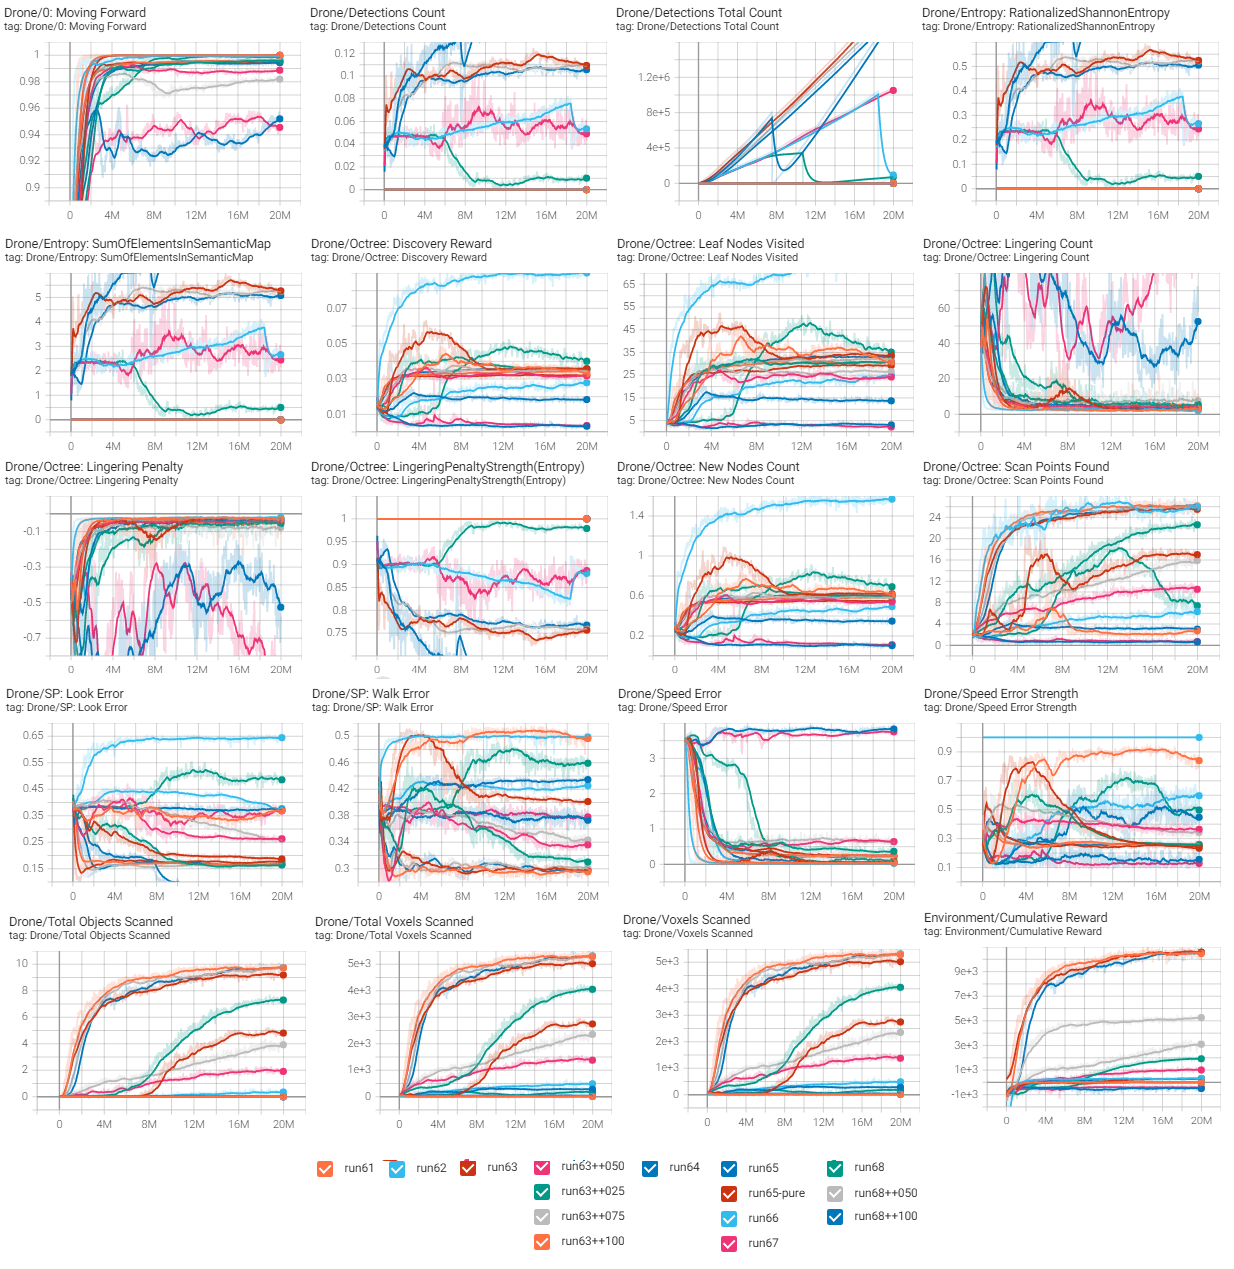
\includegraphics[width=1\textwidth]{images/results_baseAgent.png}
        \caption{Small environment (32 $m^2$) results.) .
        }
        \label{fig:results-small-env-performances}
\end{figure}

